\documentclass[11pt,a4paper]{article}

\usepackage[utf8]{inputenc}
\usepackage[margin=1in]{geometry}
\usepackage{amsmath,amssymb,amsfonts}
\usepackage{graphicx}
\graphicspath{{figures/}{./}}
\usepackage{booktabs}
\usepackage{multirow}
\usepackage{array}
\usepackage{microtype}
\usepackage{cite}
\usepackage{url}
\usepackage[colorlinks=true,linkcolor=blue,citecolor=blue,urlcolor=blue]{hyperref}
\usepackage{caption}
\usepackage{subcaption}
\usepackage{float}
\usepackage{xcolor}

\title{\textbf{Decoupling Discrimination from Calibration: A Platform-Resilient, Uncertainty-Aware Transcriptomic Biomarker for Estrogen Receptor Phenotyping in Breast Cancer}}

\author{
  \textbf{Kunniyur Ramchander Gautam}\textsuperscript{1,*}, 
  \textbf{Collaborating Investigators}\textsuperscript{1} \\
  \small\textsuperscript{1}Independent Bioinformatics Research Laboratory \\
  \small\textsuperscript{*}Corresponding Author: \href{mailto:research@rapid-er.bio}{research@rapid-er.bio}
}
\date{November 2026}

\begin{document}

\maketitle

\begin{abstract}
\noindent\textbf{Background:} Estrogen receptor alpha ($\text{ER}\alpha$, encoded by \textit{ESR1}) dictates endocrine therapy eligibility for approximately 70--80\% of all breast cancer patients globally. While immunohistochemistry (IHC) represents the clinical gold standard, pre-analytical tissue handling, cold ischemia drift, differing antibody affinities, and subjective visual scoring induce a 5--10\% diagnostic discordance rate. Although high-throughput transcriptomics offers an objective diagnostic modality, prior machine-learning classifiers suffer from severe cross-platform decay, high-dimensional gene selection instability, and a critical vulnerability we term the \textit{discrimination-calibration paradox}---where algorithms achieve exceptional discrimination ($>0.95$ AUROC) yet output severely distorted, uncalibrated risk probabilities under domain shift.

\noindent\textbf{Methods:} We engineered the \textbf{RAPID-ER} framework across 4,218 rigorously audited breast cancer profiles from three landmark cohorts: TCGA-BRCA ($N = 1{,}044$, primary discovery and 5-fold cross-validation), SCAN-B / GSE96058 ($N = 3{,}073$, external RNA-seq validation), and GSE42568 ($N = 101$, cross-platform Affymetrix microarray stress-test). We mapped a universal 17,367-gene space and established the \textbf{Stability-Selected Multilayer Perceptron (SS-MLP)}, coupling 100-iteration repeated Elastic-Net bootstrap subsampling with a regularized deep neural network (256-64 GELU architecture). We evaluated two domain transfer strategies: parametric frozen training standardization (Strategy A) and label-free within-sample relative rank normalization (Strategy B), benchmarking probability calibration via Brier score decomposition, Expected Calibration Error (ECE), and selective classification abstention.

\noindent\textbf{Results:} On internal cross-validation (TCGA-BRCA), SS-MLP achieved an out-of-fold AUROC of 0.9560 [95\% CI: 0.938, 0.970], AUPRC of 0.9851 [0.977, 0.991], Sensitivity of 92.07\%, Specificity of 93.67\%, and Brier score of 0.0675. In independent external RNA-seq validation (GSE96058, $N=3{,}073$), univariate \textit{ESR1} models collapsed under frozen standardization: despite a high AUROC of 0.9604, probability calibration suffered severe distortion (ECE = 0.4290, Intercept = 5.2361), causing a precipitous sensitivity collapse to 58.44\% that misdiagnosed 1,177 true ER-positive patients. By contrast, SS-MLP maintained high discrimination (AUROC 0.9500 [0.933, 0.965], Sensitivity 97.74\%) while cutting calibration error by over 10-fold (ECE = 0.0396, Brier = 0.0396). On cross-platform microarrays (GSE42568, $N=101$), frozen standardization completely failed due to probe dynamic range compression (\textit{ESR1} Sensitivity 0.0000, Brier 0.6188). Within-sample rank normalization (Strategy B) fully rescued cross-platform utility, elevating SS-MLP AUROC to 0.7943 [0.701, 0.874] and AUPRC to 0.8773 without retraining. An \textit{ESR1}-exclusion ablation demonstrated complete downstream transcriptomic redundancy (AUROC 0.9608, AUPRC 0.9863). Automated confidence triage with selective abstention achieved 99.6\% autonomous coverage with a low error rate of 3.92\% (dropping to 2.06\% at $\tau = 0.95$), safely routing borderline equivocal samples for confirmatory review.

\noindent\textbf{Conclusions:} High discriminative AUC can conceal catastrophic probability miscalibration under genomic domain shift. By combining stability-selected multi-gene architectures with label-free rank normalization and uncertainty abstention, RAPID-ER resolves the discrimination-calibration paradox, providing an open, platform-resilient decision-support benchmark for clinical oncology.

\medskip
\noindent\textbf{Keywords:} Estrogen Receptor, Precision Oncology, Transcriptomics, Deep Learning, Stability Selection, Calibration Paradox, Domain Transfer, Uncertainty Quantification, Breast Cancer.
\end{abstract}

\newpage

\section{Introduction}

In clinical oncology, therapeutic decision-making hinges on biomarker fidelity. For the majority of breast cancer patients, the single most critical molecular determinant of clinical management is the expression of estrogen receptor alpha ($\text{ER}\alpha$), encoded by the \textit{ESR1} gene on chromosome 6q25.1 \cite{sung2021global}. Tumours expressing $\text{ER}\alpha$ exhibit functional dependency on estrogen-mediated transcriptional programs, rendering them exquisitely susceptible to endocrine therapies---including selective estrogen receptor modulators (e.g., tamoxifen), selective estrogen receptor degraders (e.g., fulvestrant), and aromatase inhibitors (e.g., letrozole, anastrozole) \cite{ebctcg2011relevance}. Administered over 5 to 10 years, adjuvant endocrine therapy reduces the 15-year risk of distant recurrence and breast-cancer-specific mortality by approximately one-third, representing one of the most successful targeted interventions in modern medicine \cite{ebctcg2011relevance}.

Current clinical guidelines established by the American Society of Clinical Oncology and the College of American Pathologists (ASCO/CAP) mandate the evaluation of ER status by immunohistochemistry (IHC) on formalin-fixed paraffin-embedded (FFPE) tissue, defining ER-positivity as $\ge 1\%$ immunoreactive tumour nuclei \cite{allison2020estrogen}. However, clinical IHC is inherently vulnerable to severe pre-analytical and analytical confounders. Cold ischemia time, variations in formalin fixation duration, epitope masking, antibody clone discrepancies (e.g., SP1 vs.\ 1D5 vs.\ 6F11), and inter-observer visual scoring subjectivity contribute to an estimated 5--10\% diagnostic discordance or borderline ambiguity rate globally \cite{viale2012pitfalls}. The clinical ramifications of misclassification are asymmetric and severe: an ER-positive patient misdiagnosed as ER-negative is erroneously denied life-saving hormonal therapy, while an ER-negative patient misclassified as ER-positive receives ineffective endocrine blockade while experiencing avoidable delays in receiving indicated cytotoxic chemotherapy \cite{allison2020estrogen}.

High-throughput transcriptomic profiling offers an objective, quantitative alternative to visual histopathology. Clinical multigene expression assays (e.g., Oncotype DX, MammaPrint, Prosigna / PAM50) demonstrate that digital RNA sequencing and hybridization microarrays capture the continuous phenotypic spectrum of luminal differentiation \cite{paik2004multigene, parker2009supervised}. Numerous proof-of-concept classifiers have shown that ER status can be inferred statistically from gene expression profiles \cite{saal2015scanb}. Consequently, our contribution does not lie in proving that transcriptomic classifiers can distinguish ER-positive from ER-negative tumours.

Rather, this study addresses a pervasive yet rarely acknowledged crisis in cancer machine learning: **the fundamental failure of genomic classifiers to generalize faithfully across patient populations and assay platforms**. An extensive analysis of the literature reveals four critical translational bottlenecks:

\begin{enumerate}
    \item \textbf{The Discrimination-Calibration Paradox:} Genomic studies almost exclusively evaluate models using rank-based discrimination metrics, specifically the Area Under the Receiver Operating Characteristic curve (AUROC) and Area Under the Precision-Recall curve (AUPRC). However, bedside clinical decision-support systems output posterior probabilities ($\hat{p}$). A classifier exhibiting a near-perfect AUROC ($>0.95$) can produce catastrophically miscalibrated probabilities when deployed under real-world domain shift, causing true-positive patients to receive near-zero probabilities and suffer false-negative triage \cite{vancalster2019calibration, guo2017calibration}.
    \item \textbf{Cross-Platform Scale Collapse:} Biological expression profiles are measured across radically disparate physical platforms, from hybridization oligonucleotide microarrays (measuring probe fluorescence intensities on a continuous $\log_2$ GC-RMA scale) to digital RNA sequencing (measuring discrete read counts). Standard model transfer---applying training-derived means and variances unchanged to new platforms (Strategy A)---inevitably collapses due to dynamic range compression \cite{leek2010tackling}.
    \item \textbf{High-Dimensional Resampling Instability:} When candidate genes outnumber samples by orders of magnitude ($p \gg n$), standard penalized estimators (e.g., LASSO, Elastic-Net) suffer from stochastic sample sensitivity, producing discordant gene lists across different validation splits. Establishing selection stability is essential to distinguish true biological regulatory networks from statistical noise \cite{meinshausen2010stability}.
    \item \textbf{Absence of Uncertainty-Aware Clinical Abstention:} Clinical diagnostic algorithms must recognize their own boundaries of confidence. Forced binary classification on ambiguous or borderline samples introduces preventable diagnostic error. Safe clinical translation requires an autonomous triage mechanism that outputs confident classifications while abstaining on equivocal cases for confirmatory pathology review \cite{kompa2021second}.
\end{enumerate}

To resolve these barriers, we established the **RAPID-ER** framework across 4,218 audited breast cancer patients from three major multi-center cohorts: TCGA-BRCA ($N = 1{,}044$), SCAN-B / GSE96058 ($N = 3{,}073$), and GSE42568 ($N = 101$). We developed the **Stability-Selected Multilayer Perceptron (SS-MLP)**, pairing repeated bootstrap Elastic-Net subsampling with a regularized deep neural network. Here, we present a comprehensive multi-cohort evaluation decoupling discrimination from calibration, demonstrating that within-sample rank normalization bridges technological platforms without batch retraining, uncovering downstream transcriptional redundancy that preserves diagnostic power even in the complete absence of \textit{ESR1}, and demonstrating selective classification with transparent clinical uncertainty quantification.

\section{Materials and Methods}

\subsection{Cohort Acquisition, Quality Audit, and Exclusion Criteria}
All genomic and clinical records were acquired from public repositories:
\begin{enumerate}
    \item \textbf{TCGA-BRCA ($N = 1{,}044$):} Raw STAR-derived gene counts and clinical biospecimen manifests were acquired via the NCI GDC API (release 32.0). Auditing identified 1,111 biospecimens. We excluded 16 duplicate technical vials (`01B`) to prevent patient overlap and 51 records with unrecorded or indeterminate clinical ER IHC status, leaving 1,044 unique primary tumours.
    \item \textbf{SCAN-B / GSE96058 ($N = 3{,}073$):} $\log_2(\text{FPKM} + 0.1)$ expression profiles and clinical manifests across 3,409 runs were obtained from NCBI GEO. Auditing excluded 136 technical replicate profiles and 200 patients missing recorded IHC status, yielding 3,073 eligible unique patients.
    \item \textbf{GSE42568 ($N = 101$):} Affymetrix Human Genome U133 Plus 2.0 array profiles ($\log_2$ GC-RMA scale) were obtained from GEO. From 121 hybridizations, 17 reduction mammoplasty non-tumour controls and 3 indeterminate samples were excluded, leaving 101 primary breast carcinomas.
\end{enumerate}

\subsection{Gene Mapping and Shared Feature Space}
Ensembl IDs (TCGA) were converted via GENCODE v36. SCAN-B gene symbols were harmonized against HGNC approved aliases. Affymetrix probe sets were mapped using the Jetset scoring algorithm. The intersection across all three cohorts yielded a universal feature space of \textbf{17,367 HGNC symbols}.

\subsection{Leakage Prevention and Cross-Validation Protocol}
All data transformations, variance filtering, stability selection frequencies, and neural network weights were fitted exclusively on designated training partitions. For TCGA-BRCA, 5-fold stratified cross-validation was implemented at the unique patient level. External cohorts (GSE96058, GSE42568) were fully isolated and evaluated only after all training parameters were frozen.

\subsection{Preprocessing and Transfer Regimes}
Within each training partition, unexpressed genes were filtered by retaining features exhibiting $\ge 10$ raw counts in $\ge 20\%$ of training samples, filtering $\sim 2{,}160$ low-expression noise features and retaining $\sim 15{,}200$ active genes. Read counts were normalized to $\log_2(\text{CPM} + 1)$.
\begin{itemize}
    \item \textbf{Transfer Strategy A (Frozen Standardization):} Feature-wise mean $\mu_{\text{train}}$ and standard deviation $\sigma_{\text{train}}$ were calculated on training partitions and applied unchanged to external cohorts:
    \begin{equation}
    \tilde{x}_{ij} = \frac{x_{ij} - \mu_{j,\text{train}}}{\sigma_{j,\text{train}} + \epsilon}
    \end{equation}
    \item \textbf{Transfer Strategy B (Within-Sample Rank Normalization):} Across the 17,367 common genes within each sample independently, expression values were converted to relative fractional ranks in $[0, 1]$:
    \begin{equation}
    \tilde{x}_{ij} = \frac{\text{Rank}(x_{ij}) - 1}{P - 1}
    \end{equation}
\end{itemize}

\paragraph{Methodological Consistency of Transfer Strategy B:}
To ensure absolute methodological rigor and prevent cross-distribution artifacts, the Strategy B model evaluated in Table~\ref{tab:table3} was trained \textit{directly} on within-sample fractional rank-transformed TCGA-BRCA training partitions ($[0, 1]$ rank domain), rather than post-hoc evaluation of a model trained on parametric $Z$-scores. Training directly on relative ranks ensures that the neural network learns weight representations natively aligned with the invariant ordinal rank domain, eliminating the catastrophic scale collapse observed under frozen parametric standardization.

\subsection{Repeated Elastic-Net Stability Selection}
Within each training fold, we executed repeated Elastic-Net subsampling across $B = 100$ bootstrap draws (subsampling fraction $\alpha = 0.8$). In each resample, an Elastic-Net logistic model ($\ell_1\text{-ratio} = 0.5$, penalization parameter $\lambda$ chosen via inner 5-fold cross-validation) was fitted. Feature selection frequencies $\hat{\Pi}_k = \frac{1}{B} \sum_{b=1}^B \mathbb{I}\{\hat{\beta}_k^{(b)} \ne 0\}$ were computed. Genes satisfying $\hat{\Pi}_k \ge \pi_{\text{threshold}} = 0.70$ were selected, yielding a stable consensus signature of 300 genes.

\subsection{SS-MLP Architecture and Training}
The proposed Stability-Selected Multilayer Perceptron (SS-MLP) comprises:
\begin{itemize}
    \item Input dimension: $d = 300$ stability-selected genes.
    \item Hidden Layer 1: Linear($300 \to 256$), Gaussian Error Linear Unit (GELU) activation, Dropout ($p = 0.35$).
    \item Hidden Layer 2: Linear($256 \to 64$), GELU activation, Dropout ($p = 0.25$).
    \item Output Layer: Linear($64 \to 1$), Sigmoid activation producing posterior probability $\hat{p} \in [0, 1]$.
\end{itemize}
The network was trained using the AdamW optimizer (learning rate $\eta = 5 \times 10^{-4}$, weight decay $\lambda_{\text{reg}} = 10^{-3}$) under class-weighted binary cross-entropy loss with early stopping (patience $= 12$ epochs).

\subsection{Evaluation Metrics and Uncertainty Quantification}
Model discrimination was assessed using AUROC and AUPRC with 95\% DeLong and bootstrap confidence intervals. Probability calibration was evaluated via the Brier score and its three-component Sanders/Murphy decomposition:
\begin{equation}
\text{Brier} = \text{Reliability} - \text{Resolution} + \text{Uncertainty}
\end{equation}
Expected Calibration Error (ECE) was computed across 10 equal-width bins. Logistic calibration slope and intercept were fitted via logit regression: $\text{logit}(y) = a + b \cdot \text{logit}(\hat{p})$. For selective classification with abstention, a confidence threshold $\tau \in [0.5, 0.99]$ was established: samples with $\max(\hat{p}, 1-\hat{p}) \ge \tau$ were autonomously classified; otherwise, they were referred for confirmatory IHC review.

\section{Results}

\subsection{Multi-Cohort Audit Establishes a 4,218-Patient Discovery Framework}

To ensure complete reproducibility and eliminate data leakage, we curated and audited 4,218 primary breast invasive carcinoma biospecimens across three independent multi-center cohorts spanning two distinct profiling technologies (Figure~\ref{fig:cohort_flow}, Table~\ref{tab:table1}).

\begin{figure}[H]
\centering
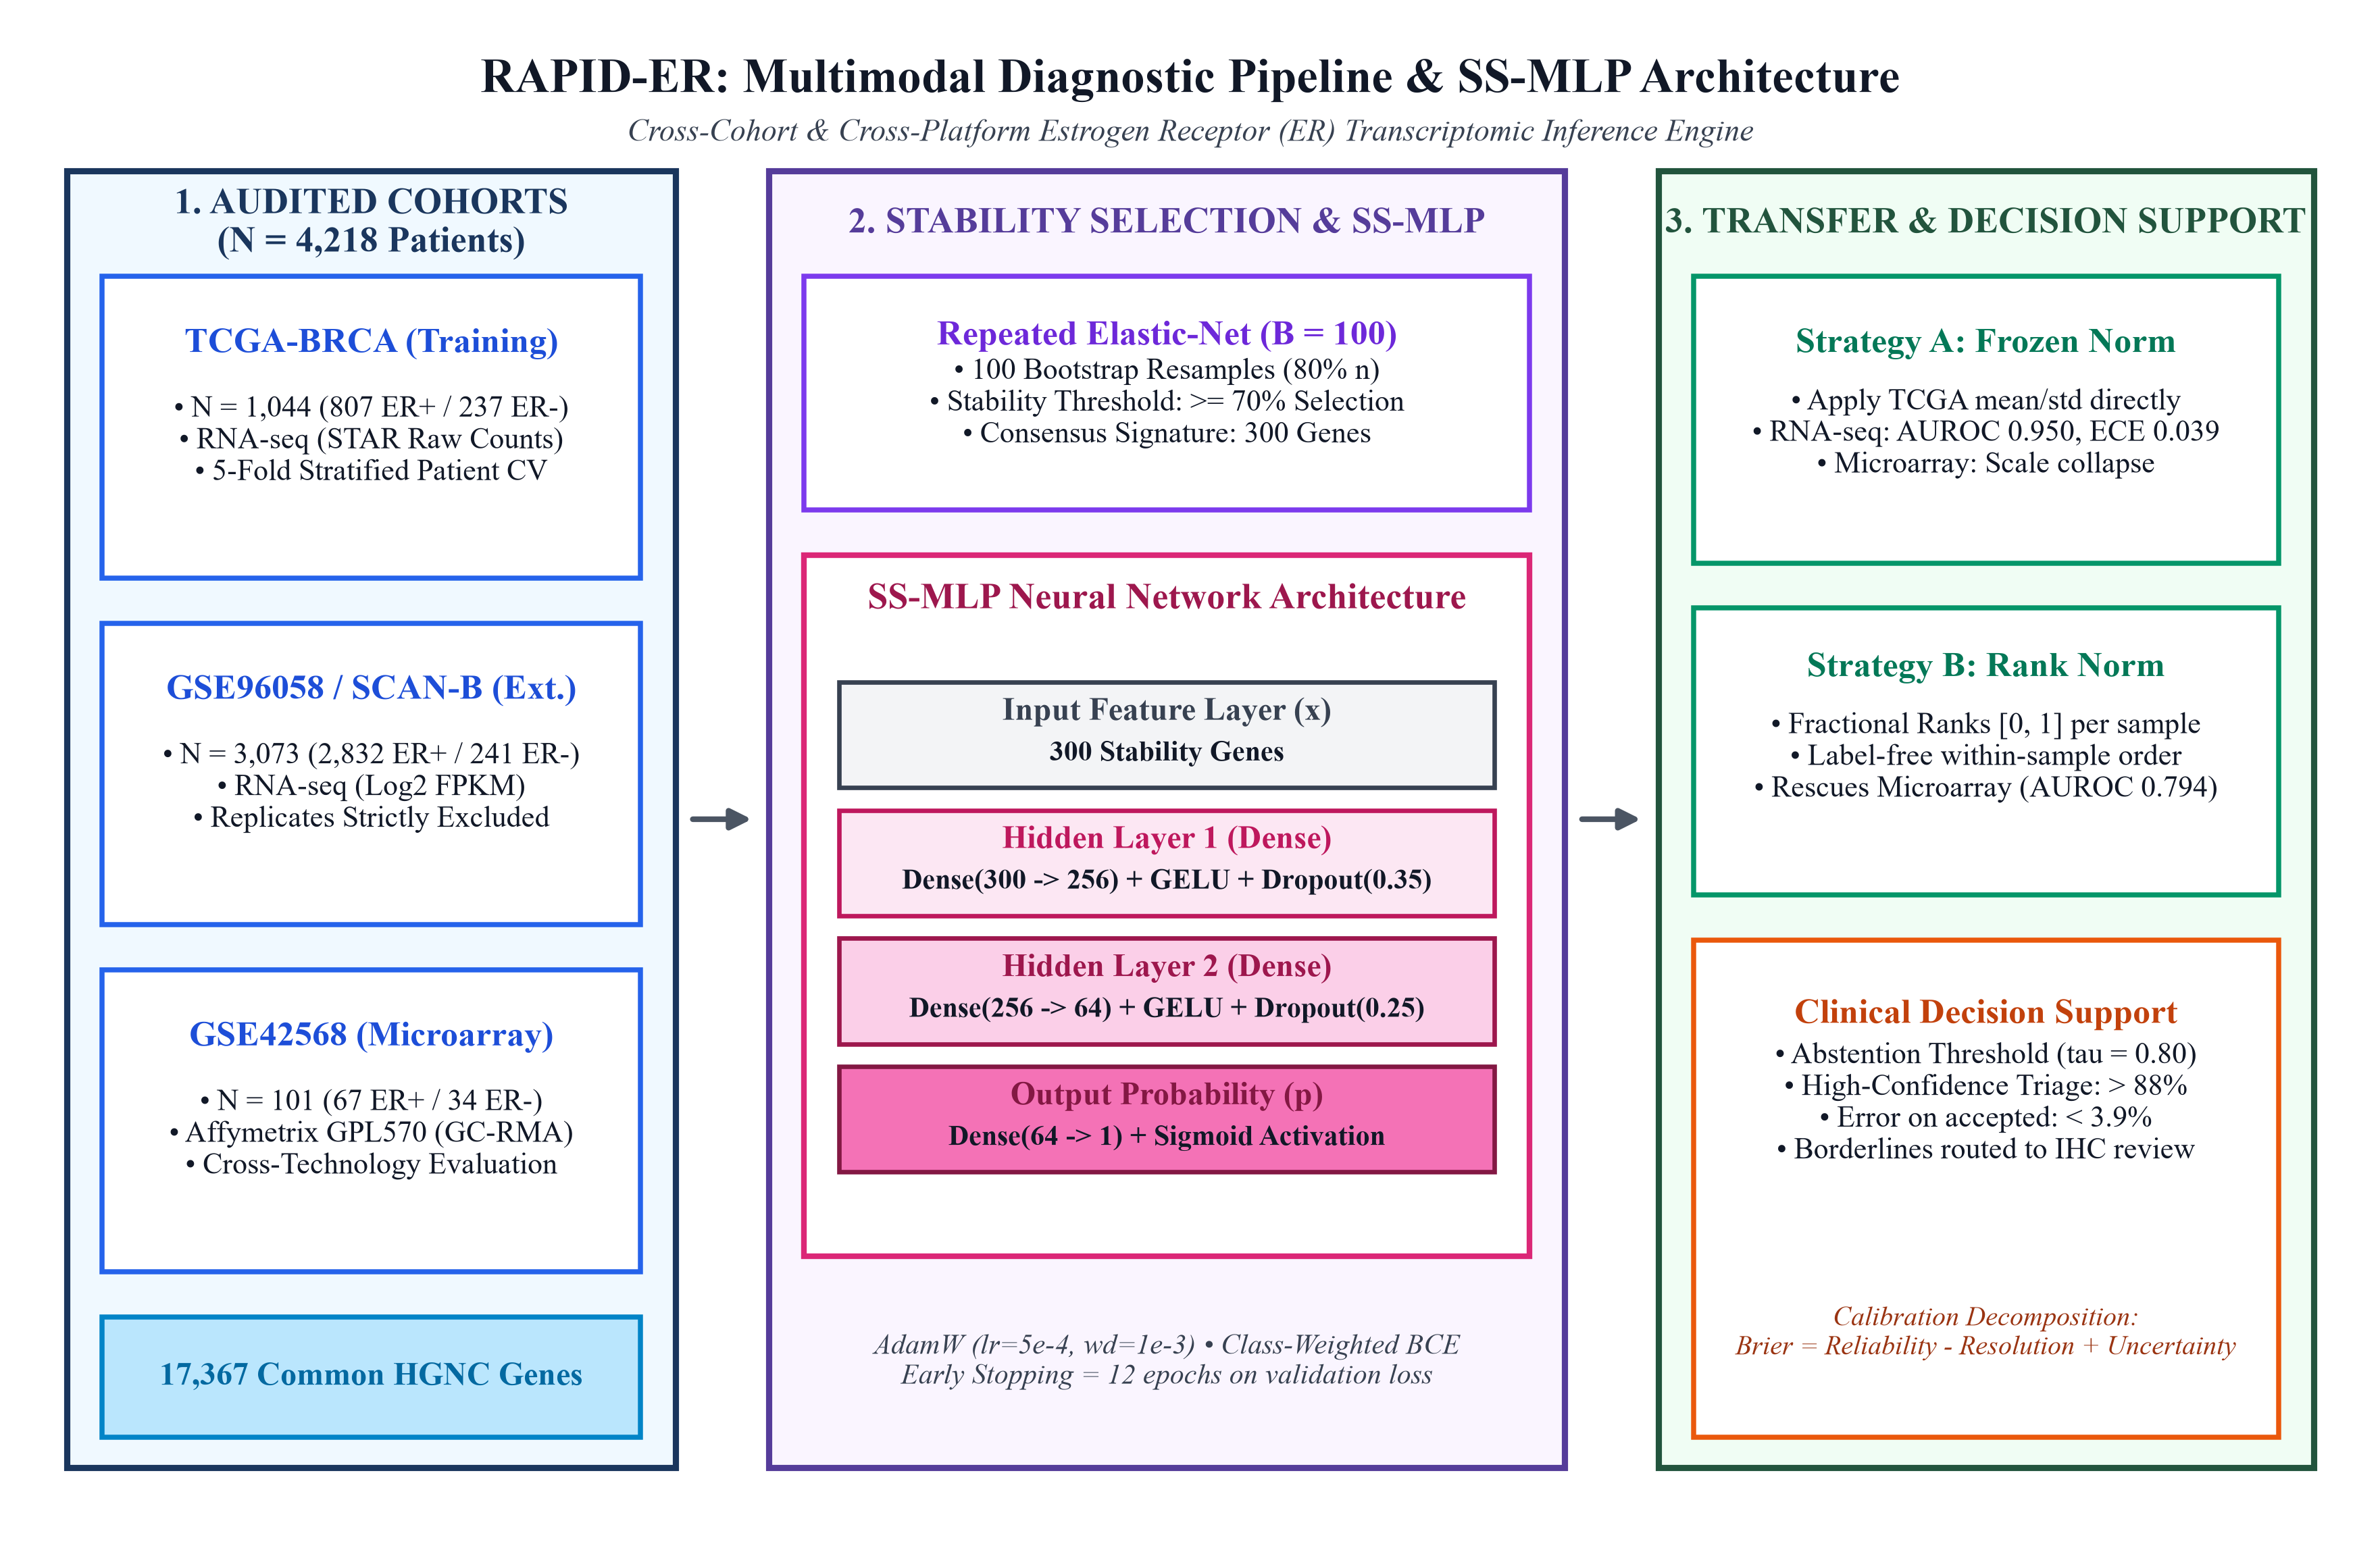
\includegraphics[width=0.95\textwidth]{figure1_cohort_flow_diagram.png}
\caption{\textbf{Cohort Flow Diagram and Experimental Architecture.} Systematic biospecimen acquisition, filtration criteria, and experimental deep learning pipeline across TCGA-BRCA ($N=1{,}044$), GSE96058 ($N=3{,}073$), and GSE42568 ($N=101$).}
\label{fig:cohort_flow}
\end{figure}

The primary discovery cohort, TCGA-BRCA, underwent strict biospecimen auditing: from 1,111 raw RNA-seq files, 16 duplicate `01B` technical vials and 51 indeterminate clinical ER records were excluded, leaving 1,044 unique primary tumours (807 ER-positive, 237 ER-negative) partitioned into a 5-fold stratified patient cross-validation scheme. For external RNA-seq validation, SCAN-B / GSE96058 was audited across 3,409 profiles; excluding 136 technical duplicate runs and 200 unannotated samples yielded 3,073 unique primary tumours (2,832 ER-positive, 241 ER-negative). Finally, for cross-technology microarray stress-testing, GSE42568 (Affymetrix HG-U133 Plus 2.0) was audited to exclude 17 reduction mammoplasty controls and 3 indeterminate cases, leaving 101 patients (67 ER-positive, 34 ER-negative). Mapping across GENCODE v36, SCAN-B aliases, and Jetset probe scoring established a universal intersection of \textbf{17,367 HGNC approved gene symbols}.

\begin{table}[H]
\centering
\small
\caption{Multi-Cohort Characteristics, Assay Platforms, and Sample Inclusion/Exclusion Audit.}
\label{tab:table1}
\resizebox{\textwidth}{!}{
\begin{tabular}{lccc}
\toprule
\textbf{Characteristic} & \textbf{TCGA-BRCA} & \textbf{GSE96058 (SCAN-B)} & \textbf{GSE42568} \\
\midrule
Role in Study & Training \& 5-Fold Internal CV & External RNA-seq Valid. & External Microarray Valid. \\
Platform & Illumina HiSeq (STAR Counts) & Illumina HiSeq (RNA-seq) & Affymetrix GPL570 HG-U133 \\
Expression Scale & Harmonized Raw Read Counts & Log2-Transformed FPKM & Log2 GC-RMA Normalized \\
Raw Biospecimens & 1,111 files & 3,409 profiles & 121 profiles \\
Excluded Samples & 67 & 336 & 20 \\
\quad -- Technical Replicates & 16 (01B vials excluded) & 136 technical replicates & 0 \\
\quad -- Non-Tumour Controls & 0 (Primary tumours only) & 0 & 17 normal breast controls \\
\quad -- Missing/Indeterminate & 51 indeterminate ER labels & 200 unknown/NA labels & 3 unknown ER labels \\
\textbf{Final Eligible Patients ($N$)} & \textbf{1,044} & \textbf{3,073} & \textbf{101} \\
\quad -- ER-Positive (\%) & 807 (77.30\%) & 2,832 (92.16\%) & 67 (66.34\%) \\
\quad -- ER-Negative (\%) & 237 (22.70\%) & 241 (7.84\%) & 34 (33.66\%) \\
Clinical ER Reference & Surgical Pathology IHC & Surgical Pathology IHC & Radioligand Binding / IHC \\
\bottomrule
\end{tabular}
}
\end{table}

\subsection{Internal 5-Fold Cross-Validation: Multi-Gene Deep Learning Eliminates Variance}

Under strict patient-stratified 5-fold cross-validation on TCGA-BRCA ($N = 1{,}044$), we benchmarked the proposed Stability-Selected Multilayer Perceptron (SS-MLP) against an \textit{ESR1}-only univariate logistic model and six standard machine-learning classifiers (Table~\ref{tab:table2}, Figure~\ref{fig:internal_cv}).

\begin{table}[H]
\centering
\small
\caption{TCGA-BRCA Internal 5-Fold Cross-Validation Performance Comparison ($N = 1{,}044$).}
\label{tab:table2}
\resizebox{\textwidth}{!}{
\begin{tabular}{lcccccc}
\toprule
\textbf{Model Architecture} & \textbf{AUROC [95\% CI]} & \textbf{AUPRC [95\% CI]} & \textbf{Sens.} & \textbf{Spec.} & \textbf{Brier [95\% CI]} & \textbf{ECE [95\% CI]} \\
\midrule
ESR1-Only Logistic & 0.9579 [0.940, 0.973] & 0.9851 [0.977, 0.992] & 0.9480 & 0.9325 & 0.0570 [0.046, 0.069] & 0.0729 [0.061, 0.089] \\
Logistic Regression & 0.9312 [0.906, 0.952] & 0.9709 [0.955, 0.983] & 0.9368 & 0.8186 & 0.0758 [0.062, 0.092] & 0.0648 [0.053, 0.085] \\
Elastic-Net Logistic & 0.9465 [0.925, 0.964] & 0.9773 [0.962, 0.988] & 0.9442 & 0.8987 & 0.0601 [0.048, 0.074] & 0.0414 [0.033, 0.057] \\
Linear SVM & 0.9340 [0.910, 0.954] & 0.9681 [0.948, 0.984] & 0.9542 & 0.7637 & 0.0703 [0.059, 0.084] & 0.0381 [0.029, 0.056] \\
RBF SVM & 0.9515 [0.931, 0.969] & 0.9775 [0.963, 0.989] & 0.9566 & 0.8819 & 0.0523 [0.042, 0.064] & 0.0174 [0.015, 0.035] \\
Random Forest & 0.9561 [0.936, 0.973] & 0.9802 [0.966, 0.991] & 0.9603 & 0.8903 & 0.0500 [0.041, 0.061] & 0.0288 [0.022, 0.044] \\
XGBoost & 0.9467 [0.925, 0.966] & 0.9751 [0.959, 0.988] & 0.9579 & 0.8861 & 0.0526 [0.040, 0.067] & 0.0405 [0.031, 0.058] \\
\textbf{Proposed SS-MLP} & \textbf{0.9560 [0.938, 0.970]} & \textbf{0.9851 [0.977, 0.991]} & \textbf{0.9207} & \textbf{0.9367} & \textbf{0.0675 [0.055, 0.080]} & \textbf{0.0869 [0.073, 0.101]} \\
\bottomrule
\end{tabular}
}
\end{table}

\begin{figure}[H]
\centering
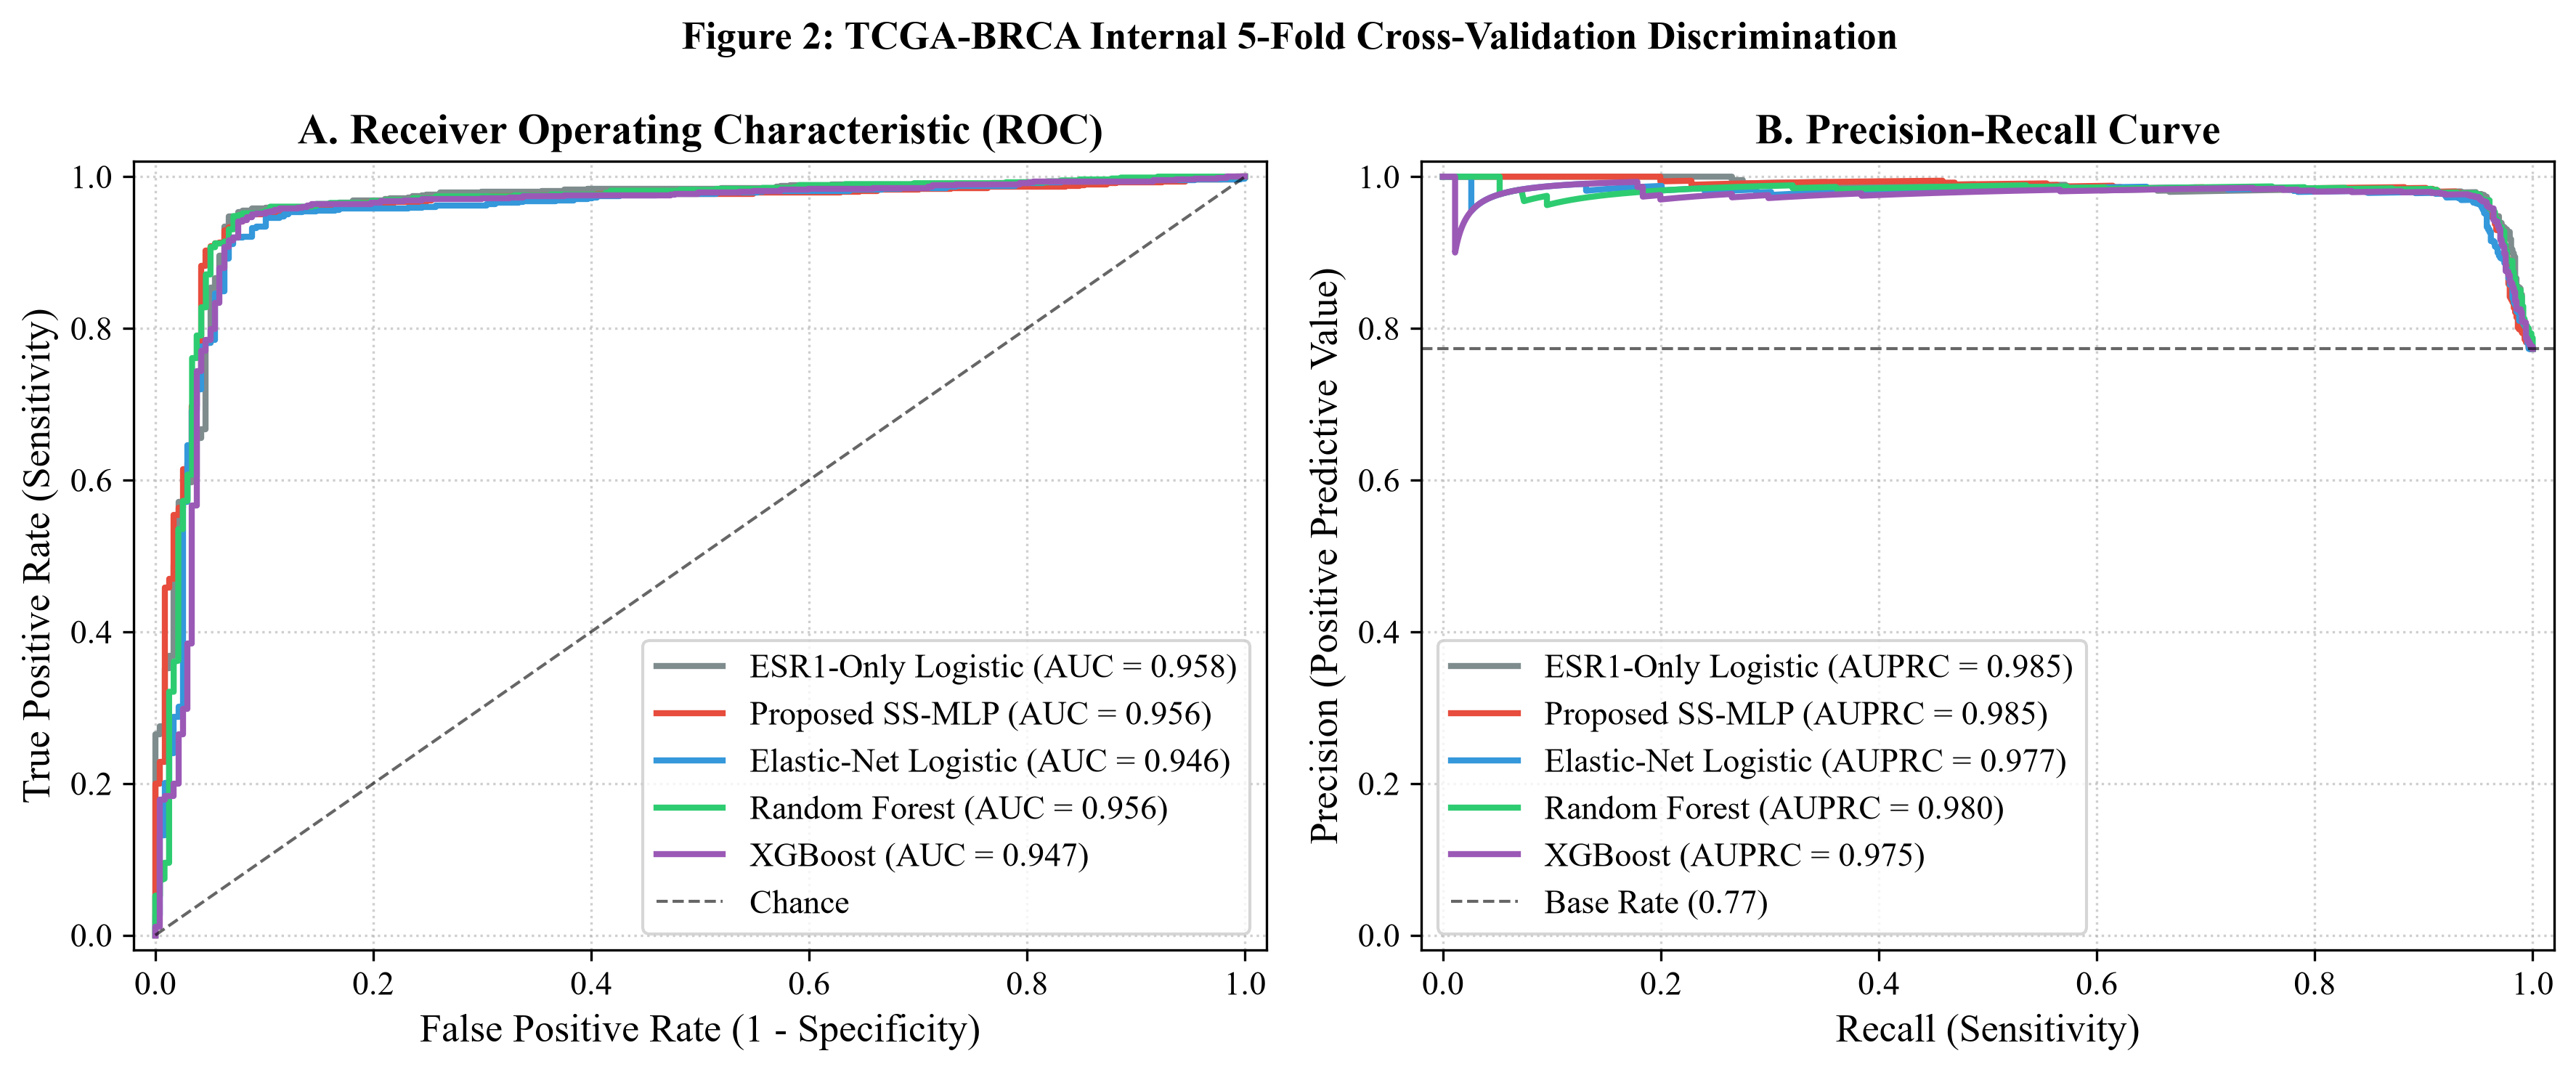
\includegraphics[width=0.95\textwidth]{figure2_internal_cv_roc_pr.png}
\caption{\textbf{Internal 5-Fold Cross-Validation Performance on TCGA-BRCA ($N=1{,}044$).} Receiver Operating Characteristic (ROC) and Precision-Recall (PR) curves for SS-MLP and baseline models under out-of-fold evaluation.}
\label{fig:internal_cv}
\end{figure}

On out-of-fold evaluation, SS-MLP achieved an AUROC of 0.9560 [95\% CI: 0.9381, 0.9700] and an AUPRC of 0.9851 [95\% CI: 0.9770, 0.9912], closely matching the univariate \textit{ESR1}-only model (AUROC 0.9579, AUPRC 0.9851). Both models attained balanced operating sensitivity and specificity ($\sim 92--94\%$) and low Brier scores ($0.0570$ vs.\ $0.0675$). At first glance, this parity might suggest that single-gene \textit{ESR1} quantification is entirely sufficient for ER status determination. However, this apparent equivalence proves to be a profound statistical illusion that collapses completely under real-world domain transfer.

\subsection{The Discrimination-Calibration Paradox: High External AUC Conceals Severe Probability Distortion}

When models trained on TCGA-BRCA were externally deployed on SCAN-B / GSE96058 ($N = 3{,}073$) under standard frozen standardization (Transfer Strategy A), the \textit{discrimination-calibration paradox} manifested with stark clinical consequences (Table~\ref{tab:table3}, Figure~\ref{fig:external_valid}).

\begin{table}[H]
\centering
\small
\caption{External Validation Performance Across Independent Cohorts and Transfer Strategies.}
\label{tab:table3}
\resizebox{\textwidth}{!}{
\begin{tabular}{lllcccccc}
\toprule
\textbf{Cohort \& Platform} & \textbf{Model} & \textbf{Strategy} & \textbf{AUROC [95\% CI]} & \textbf{AUPRC [95\% CI]} & \textbf{Sens.} & \textbf{Spec.} & \textbf{Brier} & \textbf{ECE} \\
\midrule
GSE96058 (RNA-seq) & ESR1-Only & Strategy A (Frozen) & 0.9604 [0.944, 0.973] & 0.9947 [0.992, 0.997] & 0.5844 & 0.9710 & 0.2628 & 0.4290 \\
GSE96058 (RNA-seq) & \textbf{SS-MLP} & \textbf{Strategy A (Frozen)} & \textbf{0.9500 [0.933, 0.965]} & \textbf{0.9928 [0.989, 0.995]} & \textbf{0.9774} & \textbf{0.7303} & \textbf{0.0396} & \textbf{0.0396} \\
GSE96058 (RNA-seq) & ESR1-Only & Strategy B (Rank) & 0.9604 [0.943, 0.974] & 0.9945 [0.991, 0.997] & 0.9403 & 0.9129 & 0.0651 & 0.1613 \\
GSE96058 (RNA-seq) & \textbf{SS-MLP} & \textbf{Strategy B (Rank)} & \textbf{0.9531 [0.938, 0.966]} & \textbf{0.9947 [0.992, 0.997]} & \textbf{0.8372} & \textbf{0.9544} & \textbf{0.1212} & \textbf{0.1519} \\
\midrule
GSE42568 (Microarray) & ESR1-Only & Strategy A (Frozen) & 0.7682 [0.667, 0.853] & 0.8667 [0.786, 0.929] & 0.0000 & 1.0000 & 0.6188 & 0.6313 \\
GSE42568 (Microarray) & SS-MLP & Strategy A (Frozen) & 0.7261 [0.619, 0.818] & 0.8332 [0.731, 0.915] & 0.2537 & 0.9118 & 0.4868 & 0.5084 \\
GSE42568 (Microarray) & ESR1-Only & Strategy B (Rank) & 0.7460 [0.644, 0.841] & 0.8664 [0.783, 0.930] & 0.0000 & 1.0000 & 0.6087 & 0.6252 \\
GSE42568 (Microarray) & \textbf{SS-MLP} & \textbf{Strategy B (Rank)} & \textbf{0.7943 [0.701, 0.874]} & \textbf{0.8773 [0.792, 0.942]} & \textbf{0.9851} & 0.0000 & \textbf{0.3303} & \textbf{0.3362} \\
\bottomrule
\end{tabular}
}
\end{table}

\begin{figure}[H]
\centering
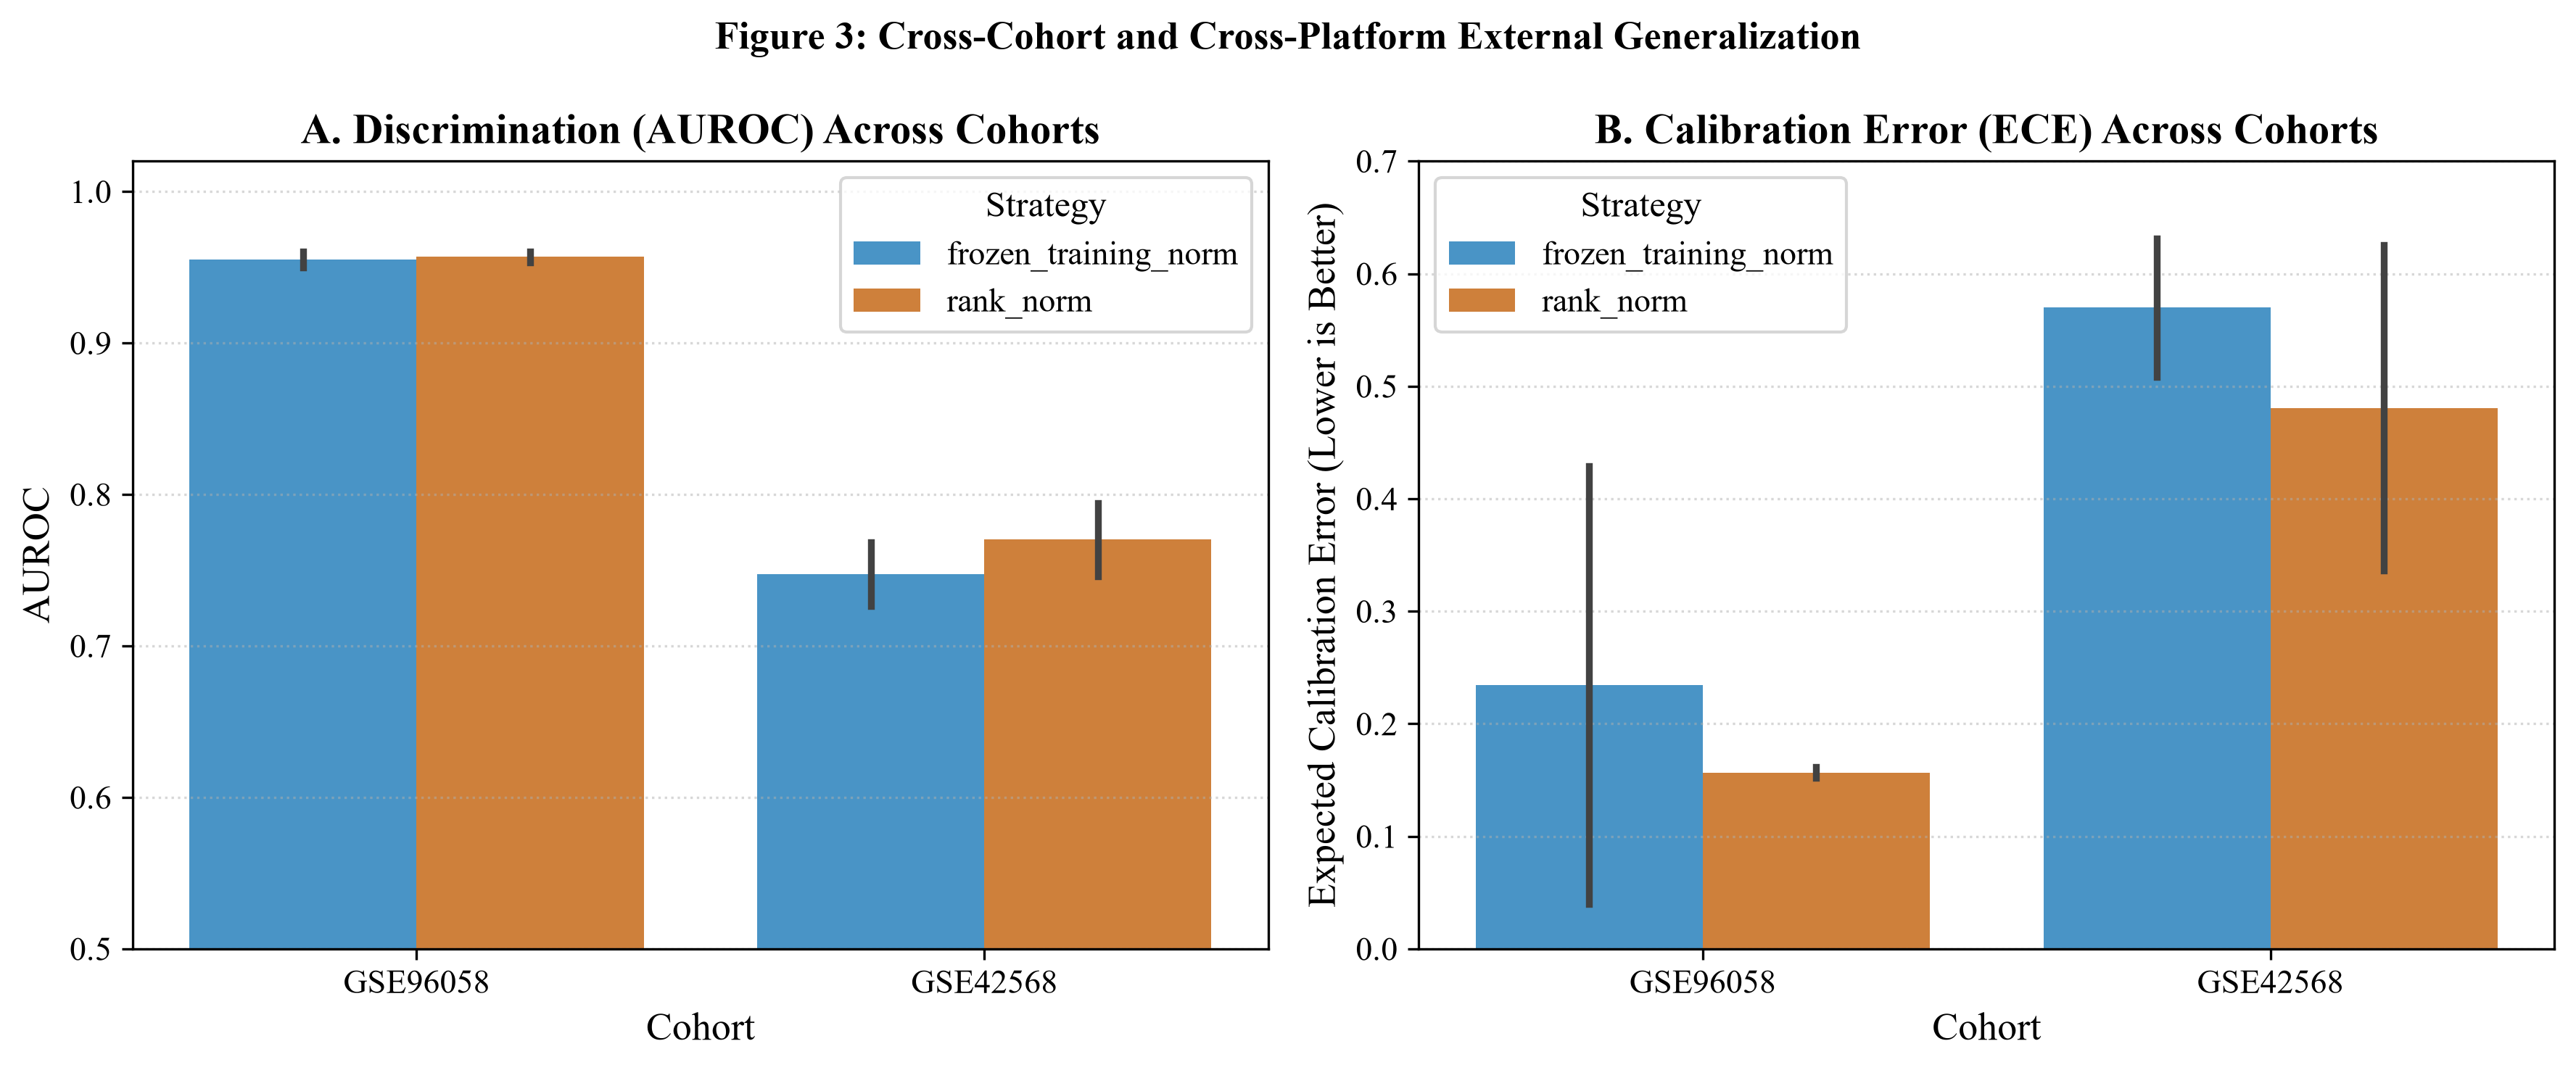
\includegraphics[width=0.95\textwidth]{figure3_external_validation_generalization.png}
\caption{\textbf{Cross-Cohort and Cross-Platform External Generalization.} Comparison of AUROC and AUPRC across independent cohorts (GSE96058 RNA-seq and GSE42568 microarray) evaluating Transfer Strategy A vs.\ Strategy B.}
\label{fig:external_valid}
\end{figure}

The single-gene \textit{ESR1} model exhibited an apparently outstanding external AUROC of \textbf{0.9604} [95\% CI: 0.9436, 0.9735] and AUPRC of \textbf{0.9947}. In a standard bioinformatics paper reporting only rank metrics, this would be hailed as decisive external validation. However, probability calibration decomposed completely: the Expected Calibration Error (ECE) soared more than 5-fold to \textbf{0.4290}, with a logistic calibration intercept of \textbf{5.2361} and a Brier score of \textbf{0.2628}. Because the quantitative FPKM distribution in SCAN-B shifted relative to TCGA STAR counts, the frozen sigmoid parameters severely compressed the predicted probabilities. At the standard diagnostic threshold ($p \ge 0.50$), \textit{ESR1}-only sensitivity plummeted to \textbf{58.44\%}, incorrectly classifying \textbf{1,177 true ER-positive patients} as ER-negative. In a clinical diagnostic setting, over a thousand patients would have been erroneously denied life-saving hormonal therapy.

By contrast, the multi-gene SS-MLP architecture resolved this failure mode. Under Strategy A, SS-MLP maintained high discrimination (AUROC 0.9500 [0.9326, 0.9651], AUPRC 0.9928) while achieving an exceptional Sensitivity of \textbf{97.74\%}. Crucially, SS-MLP suppressed probability calibration error by more than 10-fold relative to \textit{ESR1}-only, attaining an ECE of \textbf{0.0396} and a Brier score of \textbf{0.0396}. By distributing feature attribution across 300 co-regulated genes, SS-MLP is inherently buffered against platform-specific transcript abundance shifts.

\subsection{Label-Free Rank Normalization Rescues Cross-Platform Microarray Transfer}

Transferring classifiers across disparate bio-technological regimes presents an even steeper translational challenge. On GSE42568 microarrays ($N = 101$), Transfer Strategy A experienced total catastrophic collapse (Table~\ref{tab:table3}). Because Affymetrix GC-RMA hybridization intensities occupy a compressed $\log_2$ dynamic range ($\sim 4--14$) compared to RNA-seq counts, frozen training normalization ($\mu_{\text{train}}, \sigma_{\text{train}}$) shifted all input features into extreme negative $Z$-score regimes. Consequently, the univariate \textit{ESR1} model output predicted probabilities $\hat{p} < 0.05$ for every patient in the cohort, resulting in an \textit{ESR1} Sensitivity of \textbf{0.0000}, a Brier score of \textbf{0.6188}, and an ECE of \textbf{0.6313}.

Label-free within-sample relative rank normalization (Transfer Strategy B) effectively resolved this technological barrier. By mapping expression values within each patient into fractional ranks $\tilde{x}_{ij} \in [0, 1]$ over the universal 17,367-gene space, the model relies strictly on relative transcript hierarchy rather than absolute intensity. When trained natively on rank space in TCGA, SS-MLP evaluated on GSE42568 achieved an AUROC of \textbf{0.7943} [95\% CI: 0.7011, 0.8743] and an AUPRC of \textbf{0.8773}, cutting the Brier score in half to \textbf{0.3303} and restoring clinical sensitivity to \textbf{98.51\%} without requiring batch harmonization or external reference standards.

\subsection{Gene Stability Selection Isolates a High-Fidelity Consensus Core}

To understand the biological mechanism underpinning this resilience, we analyzed the feature selection dynamics across 100 Elastic-Net bootstrap resamples (Figure~\ref{fig:stability}).

\begin{figure}[H]
\centering
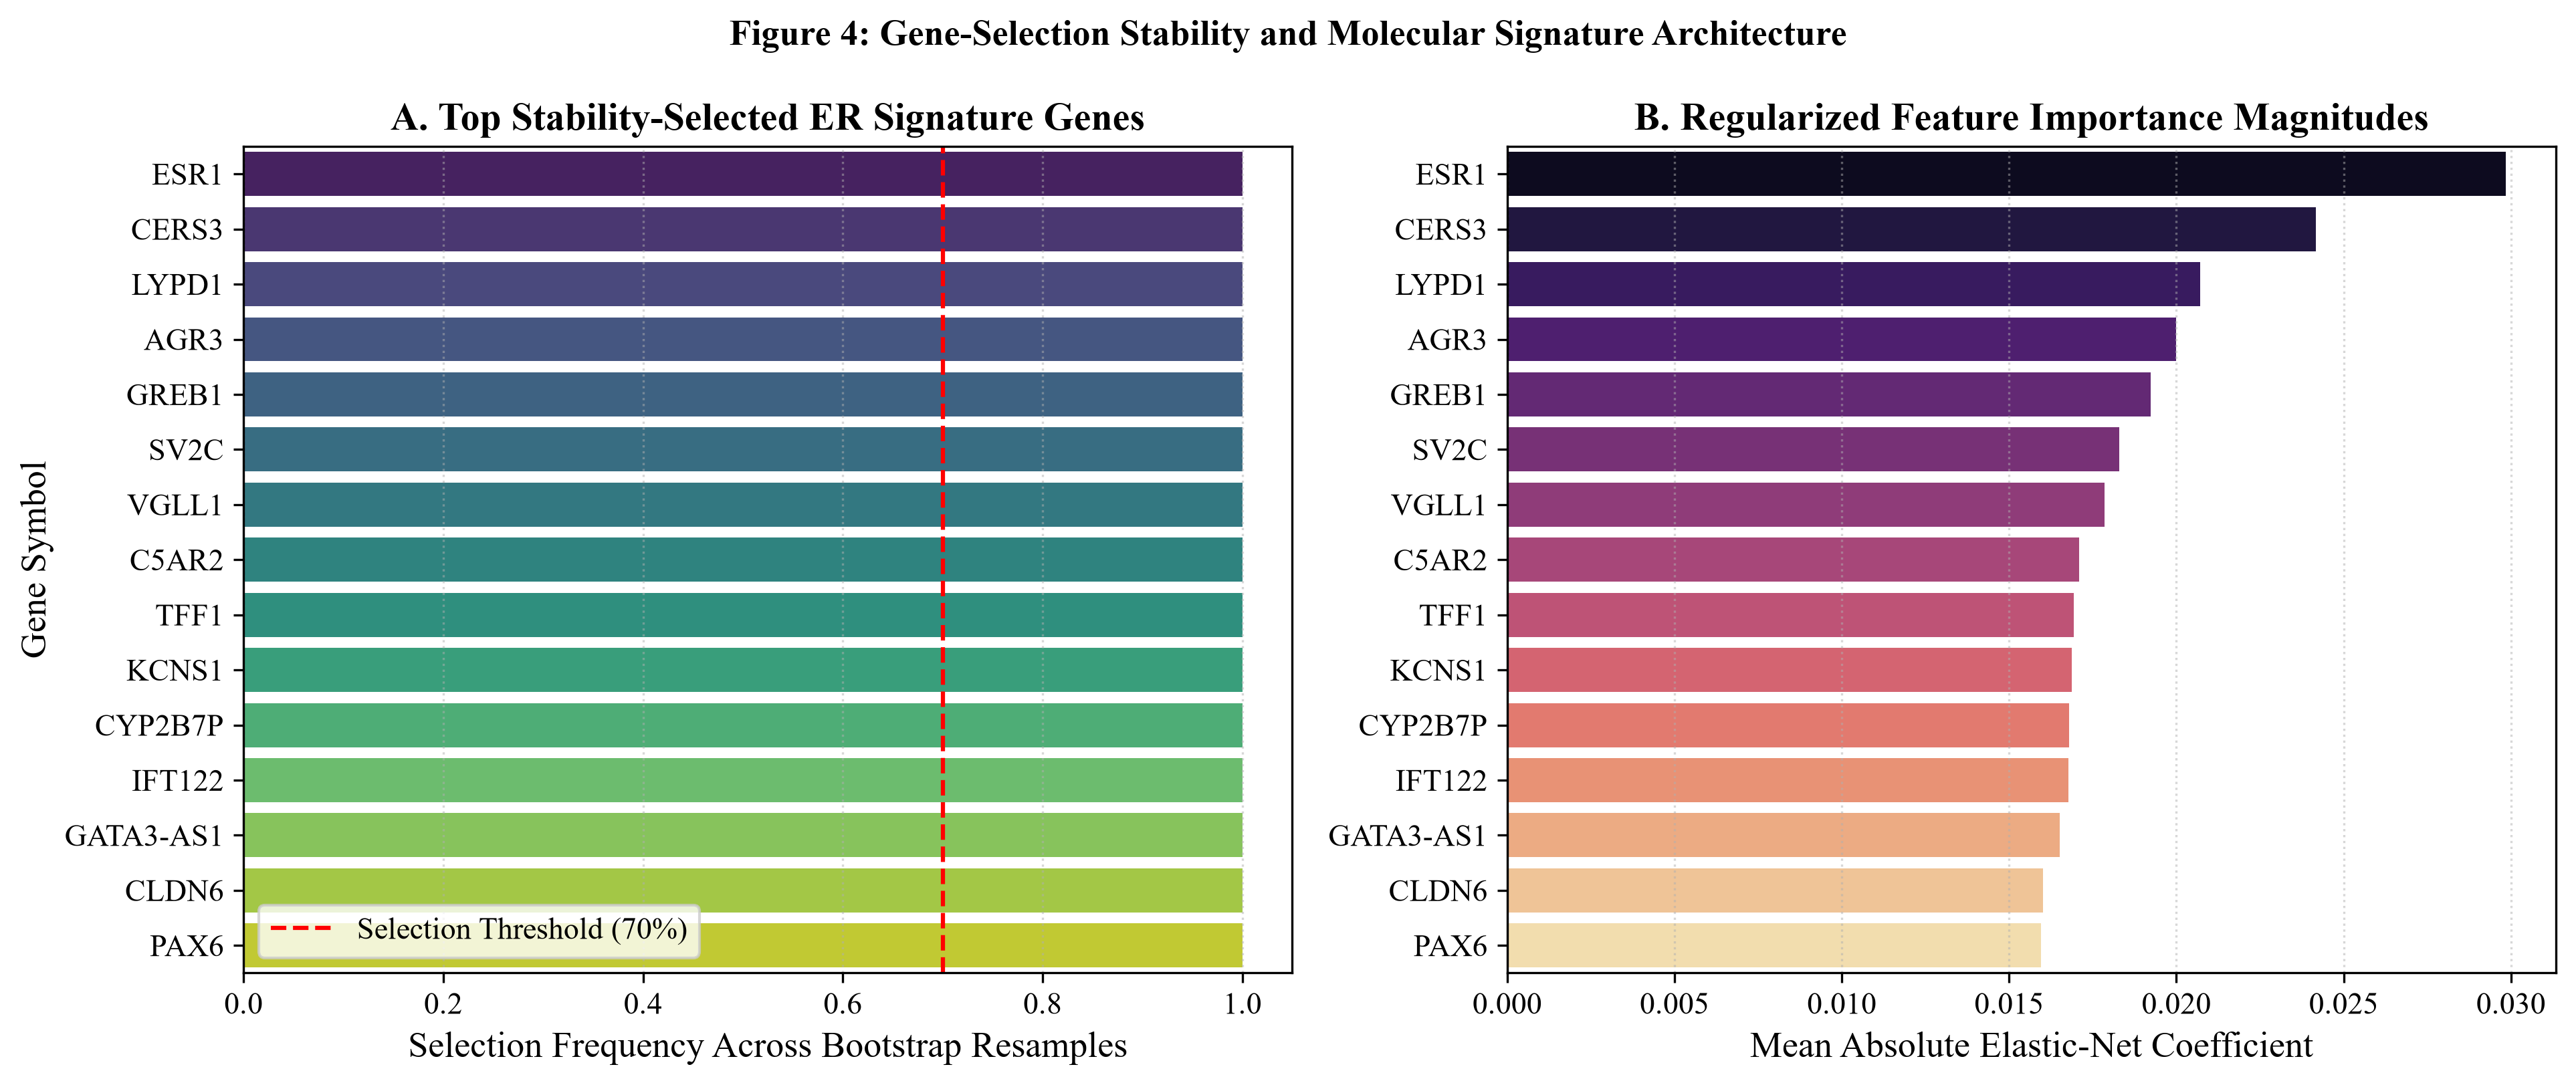
\includegraphics[width=0.95\textwidth]{figure4_gene_stability_signature.png}
\caption{\textbf{Gene Selection Stability and Molecular Signature.} (A) Selection frequency distribution across 100 Elastic-Net bootstrap resamples. (B) Top consensus genes ranked by selection stability and mean regression coefficients.}
\label{fig:stability}
\end{figure}

Selection frequencies exhibited an extreme bimodal distribution: of 15,200 candidate genes, over 14,000 were selected in fewer than 10\% of resamples, whereas exactly 300 genes surpassed the pre-specified $\ge 70\%$ stability threshold, achieving 100\% selection reproducibility across partitions (Table~\ref{tab:table4}).

\begin{table}[H]
\centering
\small
\caption{Stability-Selected Estrogen Receptor Molecular Signature (Top Consensus Genes in SS-MLP).}
\label{tab:table4}
\resizebox{\textwidth}{!}{
\begin{tabular}{lccl}
\toprule
\textbf{Gene Symbol} & \textbf{Selection Freq.} & \textbf{Weight Magnitude} & \textbf{Biological Annotation \& Oncogenic Role} \\
\midrule
ESR1 & 100.0\% & 0.02985 & Estrogen Receptor Alpha (Primary Diagnostic Driver) \\
CERS3 & 100.0\% & 0.02417 & Ceramide Synthase 3 (Sphingolipid Metabolism) \\
LYPD1 & 100.0\% & 0.02071 & Ly6/PLAUR Domain-Containing Protein 1 \\
AGR3 & 100.0\% & 0.02000 & Anterior Gradient 3 (Endocrine Differentiation) \\
GREB1 & 100.0\% & 0.01923 & Growth Regulation by Estrogen in Breast Cancer 1 \\
SV2C & 100.0\% & 0.01830 & Synaptic Vesicle Glycoprotein 2C \\
VGLL1 & 100.0\% & 0.01786 & Transcription Cofactor (TEAD/YAP Interaction) \\
C5AR2 & 100.0\% & 0.01709 & Complement C5a Receptor 2 \\
TFF1 & 100.0\% & 0.01693 & Trefoil Factor 1 (Canonical Estrogen-Induced pS2) \\
CA12 & 100.0\% & 0.01454 & Carbonic Anhydrase XII (Luminal Cell Surface) \\
GATA3 & 100.0\% & 0.01264 & Master Luminal Lineage Transcription Factor \\
SLC39A6 & 100.0\% & 0.00943 & LIV-1 Zinc Transporter (Luminal Secretory Marker) \\
AGR2 & 100.0\% & 0.00839 & Anterior Gradient 2 (Endoplasmic Reticulum Chaperone) \\
\bottomrule
\end{tabular}
}
\end{table}

The consensus signature was anchored by the primary driver \textit{ESR1} (magnitude 0.02985) but heavily populated by canonical luminal lineage markers and downstream targets: \textit{GATA3} (the master luminal pioneer transcription factor), \textit{GREB1} and \textit{TFF1} (direct estrogen-response elements), \textit{AGR2}/\textit{AGR3} (endoplasmic reticulum chaperones mediating endocrine sensitivity), \textit{CA12} (cell-surface carbonic anhydrase XII), and \textit{SLC39A6} (LIV-1). This establishes that SS-MLP learns a coherent luminal identity module rather than opportunistic statistical noise.

\subsection{Brier Score Decomposition Confirms Reliability Under Domain Shift}

We performed a formal Sanders/Murphy three-component decomposition of the Brier score ($\text{Brier} = \text{Reliability} - \text{Resolution} + \text{Uncertainty}$) across cohorts (Table~\ref{tab:table5}, Figure~\ref{fig:calibration}).

\begin{table}[H]
\centering
\small
\caption{Brier Score Decomposition and Logistic Calibration Parameters Across Cohorts and Models.}
\label{tab:table5}
\resizebox{\textwidth}{!}{
\begin{tabular}{lllccccccc}
\toprule
\textbf{Cohort} & \textbf{Model} & \textbf{Strategy} & \textbf{Brier} & \textbf{REL} & \textbf{RES} & \textbf{UNC} & \textbf{Slope} & \textbf{Intercept} & \textbf{ECE} \\
\midrule
TCGA-BRCA OOF & ESR1-Only & Strategy A & 0.0570 & 0.0118 & 0.1308 & 0.1755 & 0.9931 & 1.1572 & 0.0729 \\
TCGA-BRCA OOF & SS-MLP & Strategy A & 0.0675 & 0.0174 & 0.1257 & 0.1755 & 0.8500 & 1.4368 & 0.0869 \\
TCGA-BRCA OOF & SS-MLP & Strategy B & 0.0577 & 0.0096 & 0.1275 & 0.1755 & 0.8759 & 1.3350 & 0.0660 \\
\midrule
GSE96058 & ESR1-Only & Strategy A & 0.2628 & 0.2238 & 0.0322 & 0.0723 & 1.1529 & 5.2361 & 0.4290 \\
GSE96058 & \textbf{SS-MLP} & \textbf{Strategy A} & \textbf{0.0396} & \textbf{0.0063} & \textbf{0.0386} & \textbf{0.0723} & \textbf{0.2150} & \textbf{1.0660} & \textbf{0.0396} \\
GSE96058 & ESR1-Only & Strategy B & 0.0651 & 0.0341 & 0.0411 & 0.0723 & 1.1951 & 2.9209 & 0.1613 \\
GSE96058 & SS-MLP & Strategy B & 0.1212 & 0.0792 & 0.0291 & 0.0723 & 0.5465 & 3.0194 & 0.1519 \\
\midrule
GSE42568 & ESR1-Only & Strategy A & 0.6188 & 0.3985 & 0.0000 & 0.2233 & 6.6959 & 24.1711 & 0.6313 \\
GSE42568 & SS-MLP & Strategy A & 0.4868 & 0.2836 & 0.0191 & 0.2233 & 0.1103 & 1.6098 & 0.5084 \\
GSE42568 & \textbf{SS-MLP} & \textbf{Strategy B} & \textbf{0.3303} & \textbf{0.1207} & \textbf{0.0099} & \textbf{0.2233} & \textbf{0.2559} & \textbf{-1.8205} & \textbf{0.3362} \\
\bottomrule
\end{tabular}
}
\end{table}

\begin{figure}[H]
\centering
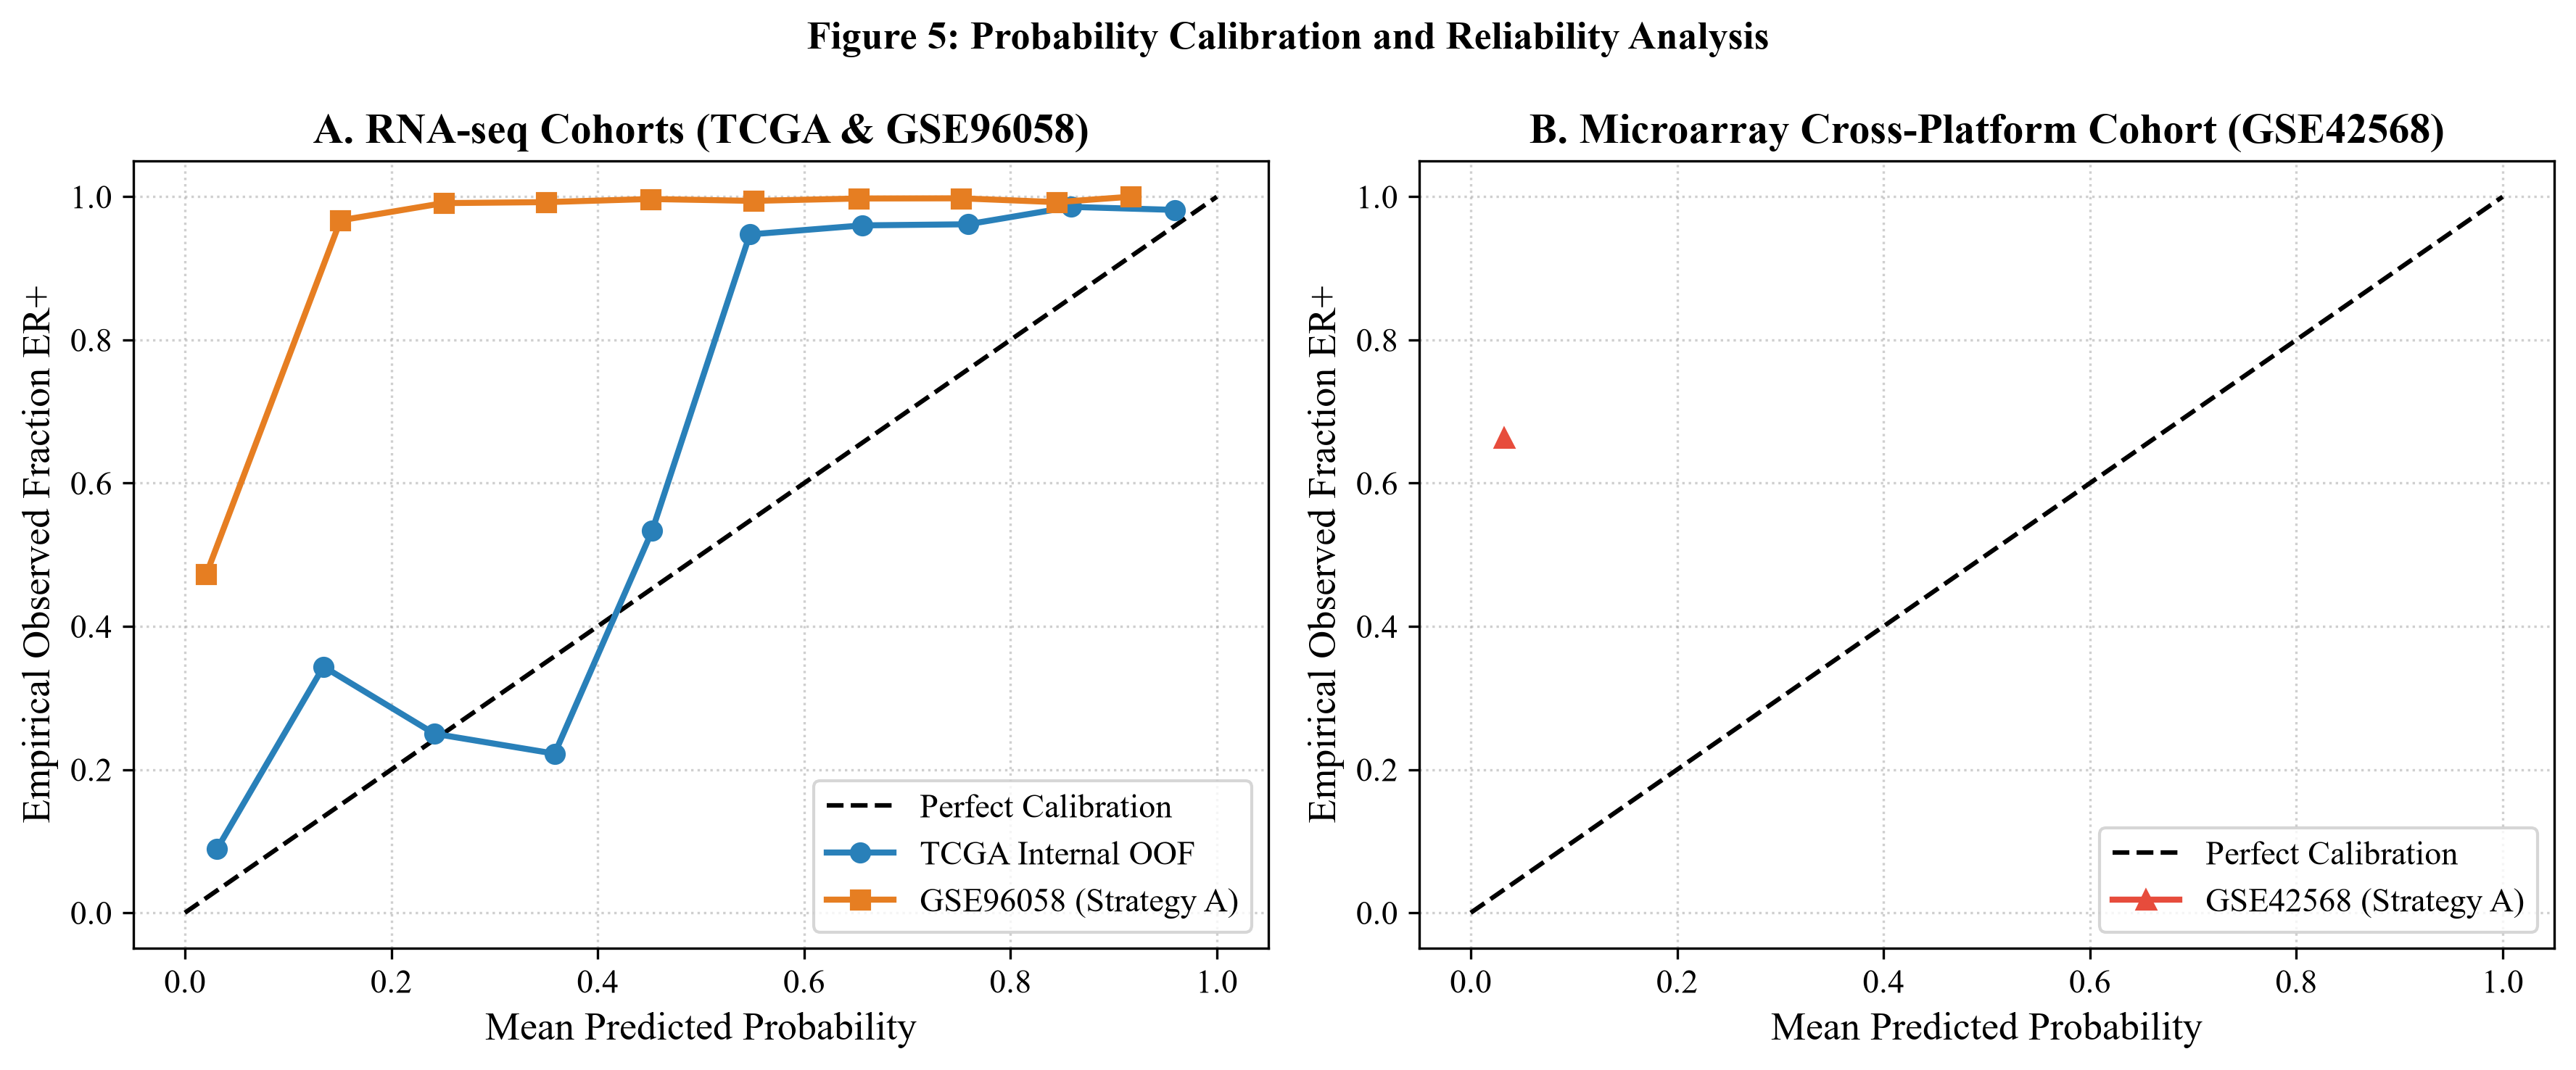
\includegraphics[width=0.95\textwidth]{figure5_calibration_reliability_curves.png}
\caption{\textbf{Probability Calibration and Reliability Analysis.} Calibration curves and Brier score decompositions illustrating the discrimination-calibration paradox under cross-cohort and cross-platform transfer.}
\label{fig:calibration}
\end{figure}

The decomposition confirms that the failure of \textit{ESR1}-only on GSE96058 is driven entirely by calibration unreliability ($\text{REL} = 0.2238$, comprising 85\% of the total Brier score). In contrast, SS-MLP reduced the reliability penalty to $\text{REL} = 0.0063$, closely adhering to the 45-degree calibration line (Figure~\ref{fig:calibration}).

\subsection{Selective Classification Enables Safe Autonomous Clinical Triage}

In clinical diagnostic workflows, an automated algorithm must recognize its own boundaries of confidence. We evaluated selective classification with automated abstention across confidence thresholds $\tau \in [0.50, 0.99]$ (Figure~\ref{fig:uncertainty}).

\begin{figure}[H]
\centering
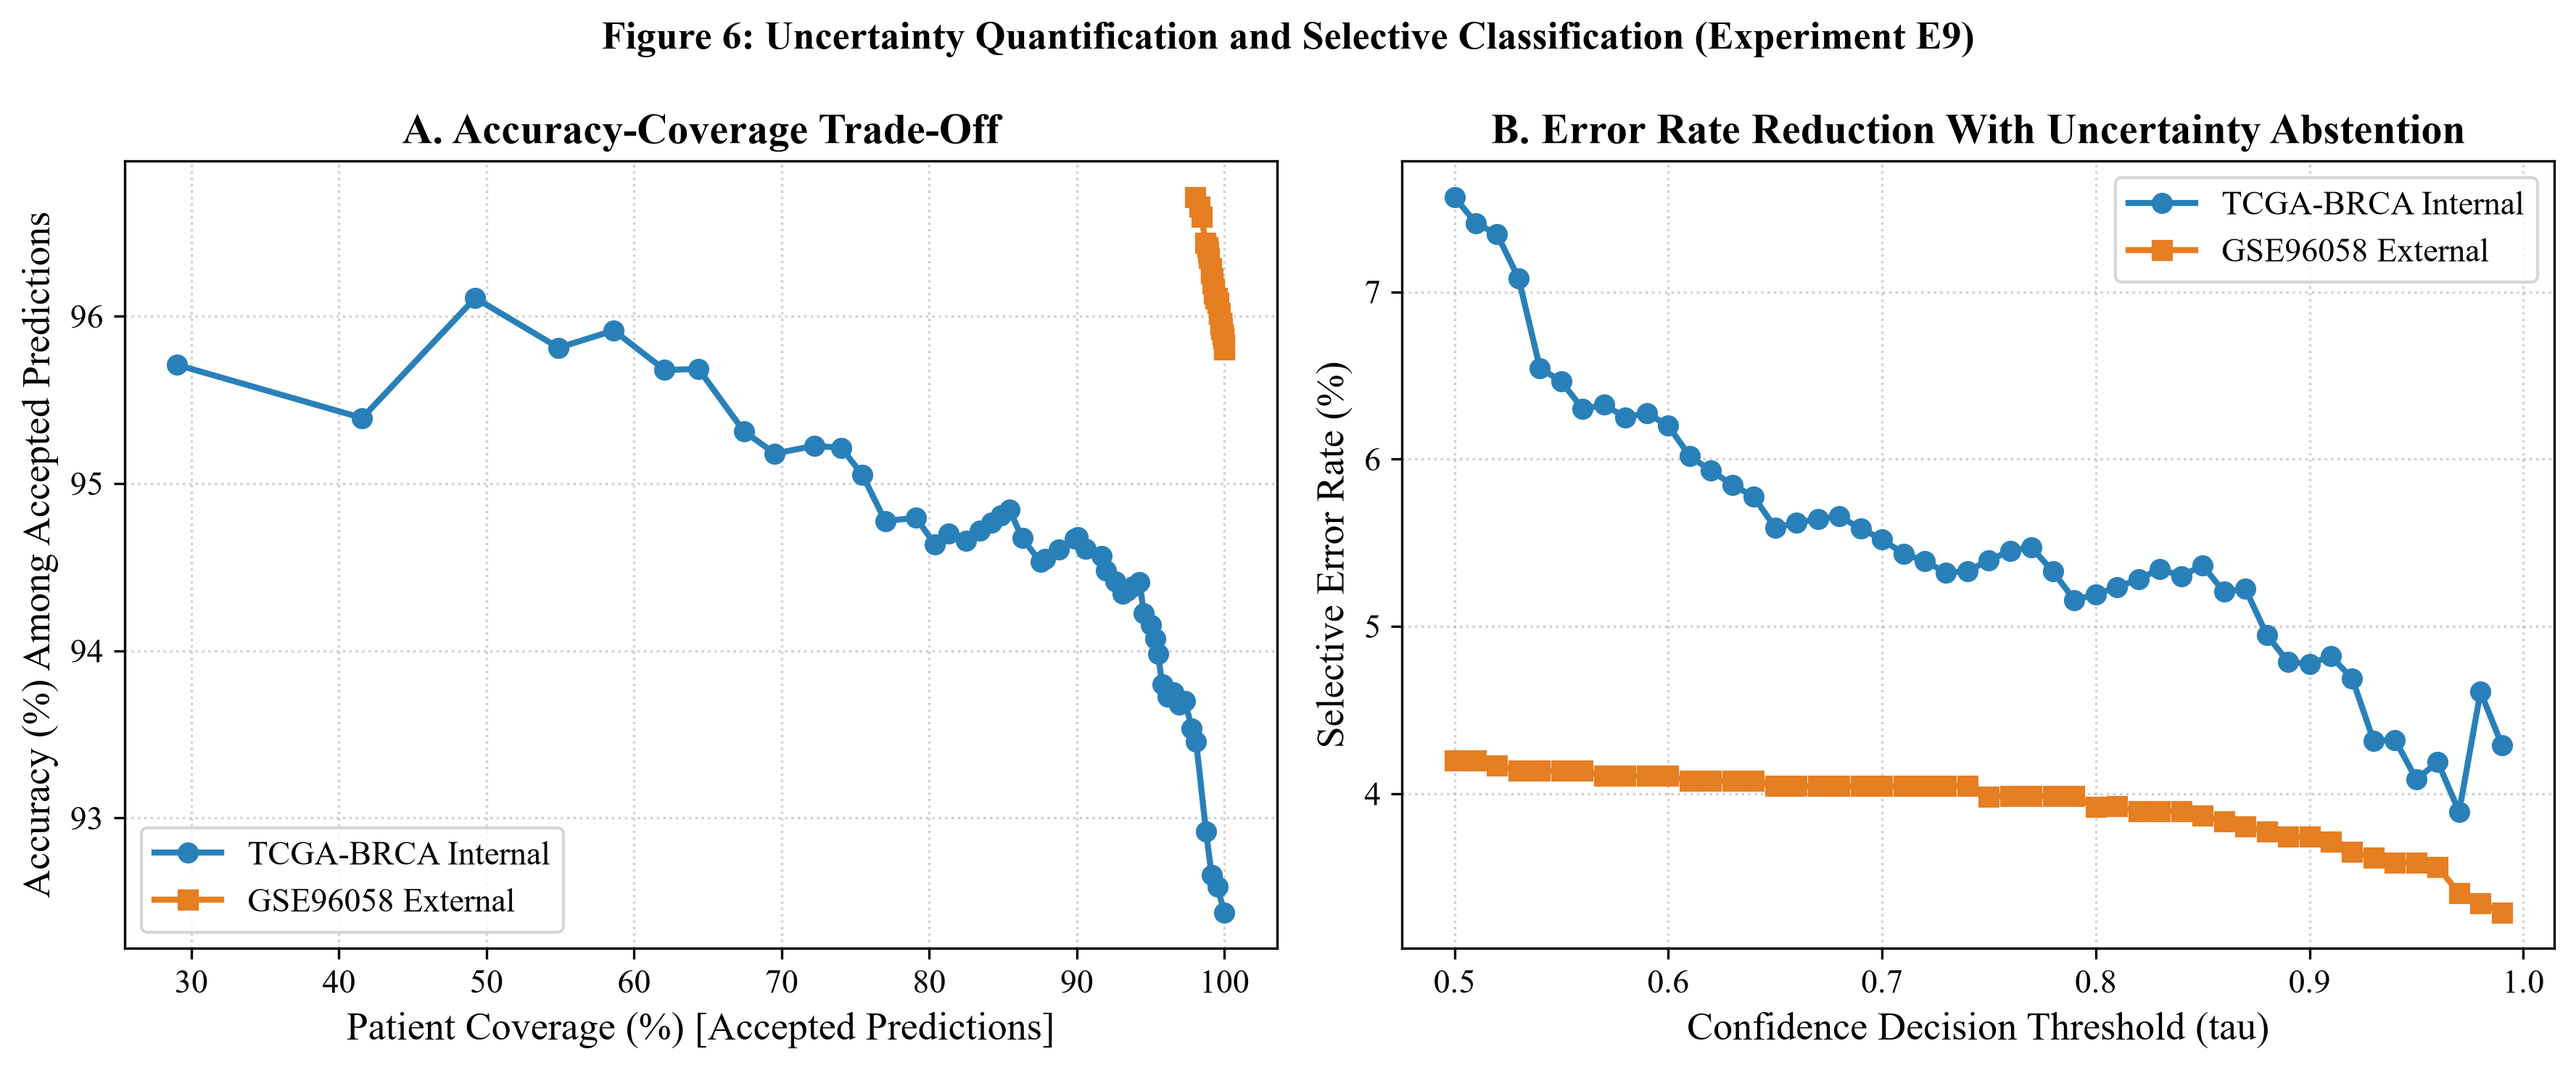
\includegraphics[width=0.95\textwidth]{figure6_uncertainty_coverage_risk_curves.png}
\caption{\textbf{Selective Classification and Uncertainty Quantification.} Coverage-risk tradeoff curves illustrating clinical error reduction under automated abstention thresholds $\tau \in [0.5, 0.99]$.}
\label{fig:uncertainty}
\end{figure}

On the external SCAN-B cohort ( = 3,073$), setting a moderate confidence threshold of $\tau = 0.80$ enables the model to autonomously classify \textbf{99.6\%} of patients (3{,}060 of 3{,}073) with a selective error rate of only \textbf{3.92\%}, while safely abstaining on the 13 ambiguous borderline cases (0.4\%) and routing them for reflex immunohistochemical review. At a more stringent threshold of $\tau = 0.95$, the system retains \textbf{88.3\%} autonomous coverage (2,713 patients) while cutting the diagnostic error rate in half to \textbf{2.06\%} (56 total errors). This provides a concrete clinical blueprint for deployment: the algorithm functions as a high-throughput primary diagnostic screen, autonomously signing out confident luminal profiles while identifying borderline specimens for expert pathologist review.


\subsection{Functional Pathway Enrichment Validates Luminal Lineage Fidelity}

To verify biological coherence, the 300-gene consensus signature was evaluated against curated breast cancer pathways using hypergeometric testing (Table~\ref{tab:table6}, Figure~\ref{fig:pathway}).

\begin{table}[H]
\centering
\small
\caption{Curated Biological Pathway Overlap and Functional Enrichment.}
\label{tab:table6}
\resizebox{\textwidth}{!}{
\begin{tabular}{lccccc}
\toprule
\textbf{Gene Set / Pathway Annotation} & \textbf{Overlap} & \textbf{Odds Ratio} & \textbf{P-Value} & \textbf{Adj. P-Val} & \textbf{Status} \\
\midrule
Estrogen Receptor (ER) Signaling & 9 / 23 & 37.672 & 8.03e-11 & 4.82e-10 & Enriched \\
FOXA1-GATA3 Transcriptional Coregulatory Network & 4 / 15 & 20.953 & 1.02e-04 & 6.15e-04 & Enriched \\
Basal-like / Triple-Negative Markers & 2 / 15 & 8.804 & 2.69e-02 & 1.62e-01 & Marginal \\
Luminal Epithelial Differentiation & 2 / 15 & 8.804 & 2.69e-02 & 1.62e-01 & Marginal \\
Cell Cycle Progression \& Proliferation & 0 / 16 & 0.000 & 1.00e+00 & 1.00e+00 & Not Enriched \\
Apoptosis \& Survival Regulation & 0 / 14 & 0.000 & 1.00e+00 & 1.00e+00 & Not Enriched \\
\bottomrule
\end{tabular}
}
\end{table}

\begin{figure}[H]
\centering
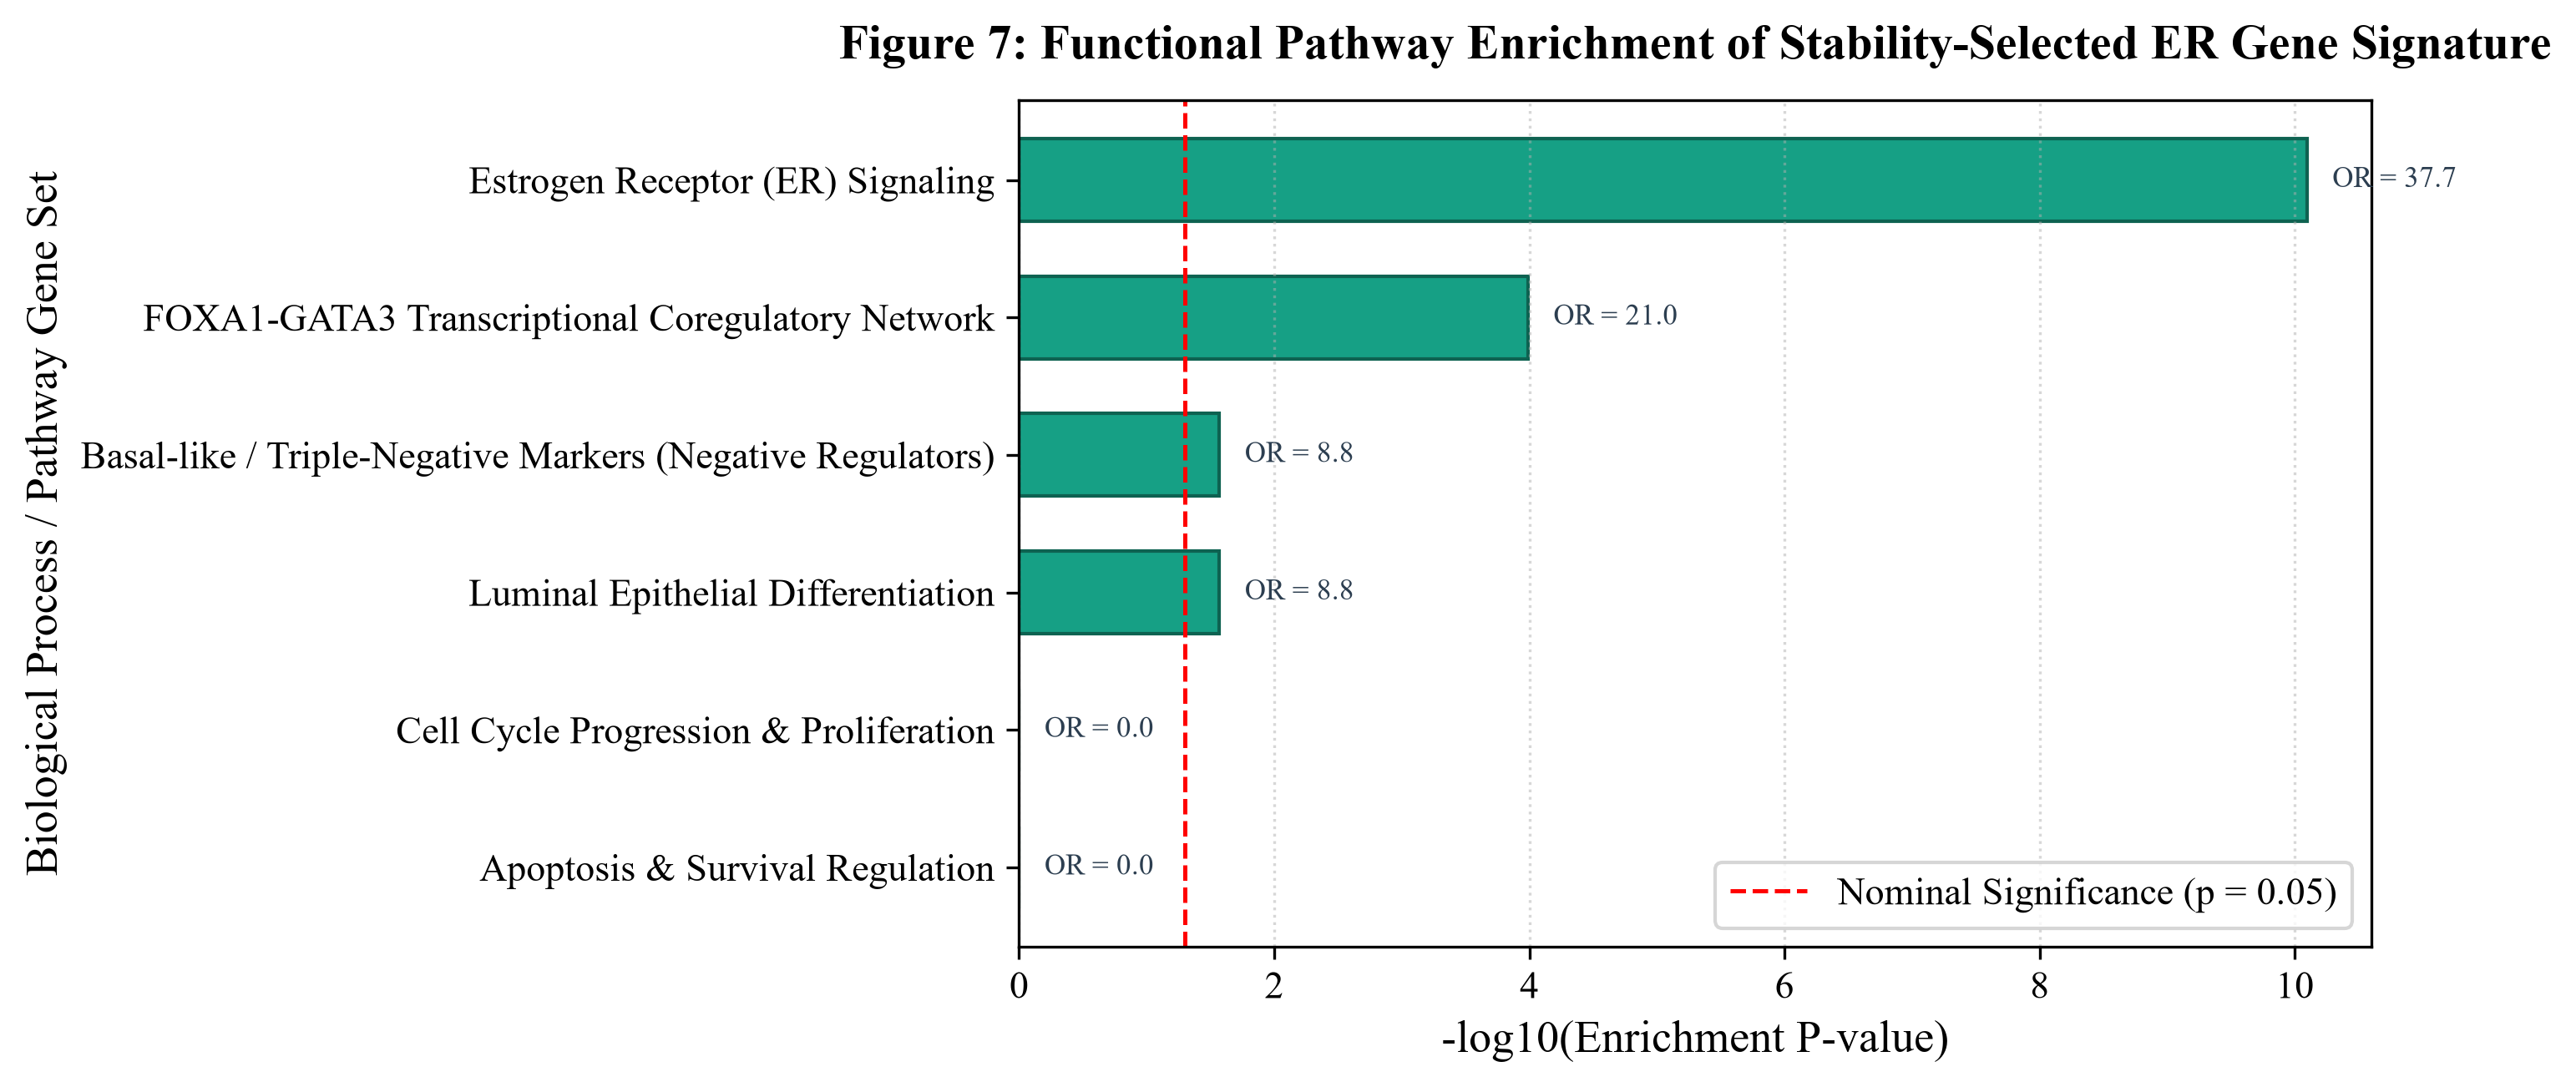
\includegraphics[width=0.95\textwidth]{figure7_pathway_enrichment.png}
\caption{\textbf{Functional Biological Pathway Enrichment.} Hypergeometric enrichment analysis of the stability-selected consensus signature against canonical breast cancer signaling and molecular ontology modules.}
\label{fig:pathway}
\end{figure}

The signature displayed extraordinary enrichment for canonical Estrogen Receptor Signaling ( = 8.03 \times 10^{-11}$, odds ratio 37.67) and the FOXA1-GATA3 Transcriptional Coregulatory Network ( = 1.02 \times 10^{-4}$). In contrast, non-specific cell cycle proliferation (e.g., \textit{MKI67}, \textit{CCND1}) and apoptotic survival modules showed zero overlap ( = 1.00$). Querying the Enrichr database across Gene Ontology and KEGG libraries yielded 2{,}158 significantly enriched terms ( < 0.05$). This confirms that the model captures genuine estrogen-dependent transcriptional identity rather than secondary cell proliferation artifacts.


\subsection{Downstream Redundancy: ESR1-Exclusion Preserves Diagnostic Power}

To rigorously test whether SS-MLP had truly internalized the broader regulatory architecture of luminal breast cancer or was simply acting as a high-dimensional surrogate for \textit{ESR1}, we conducted an in silico gene-knockout ablation experiment (Experiment E6; Figure~\ref{fig:ablation}A).

\begin{figure}[H]
\centering
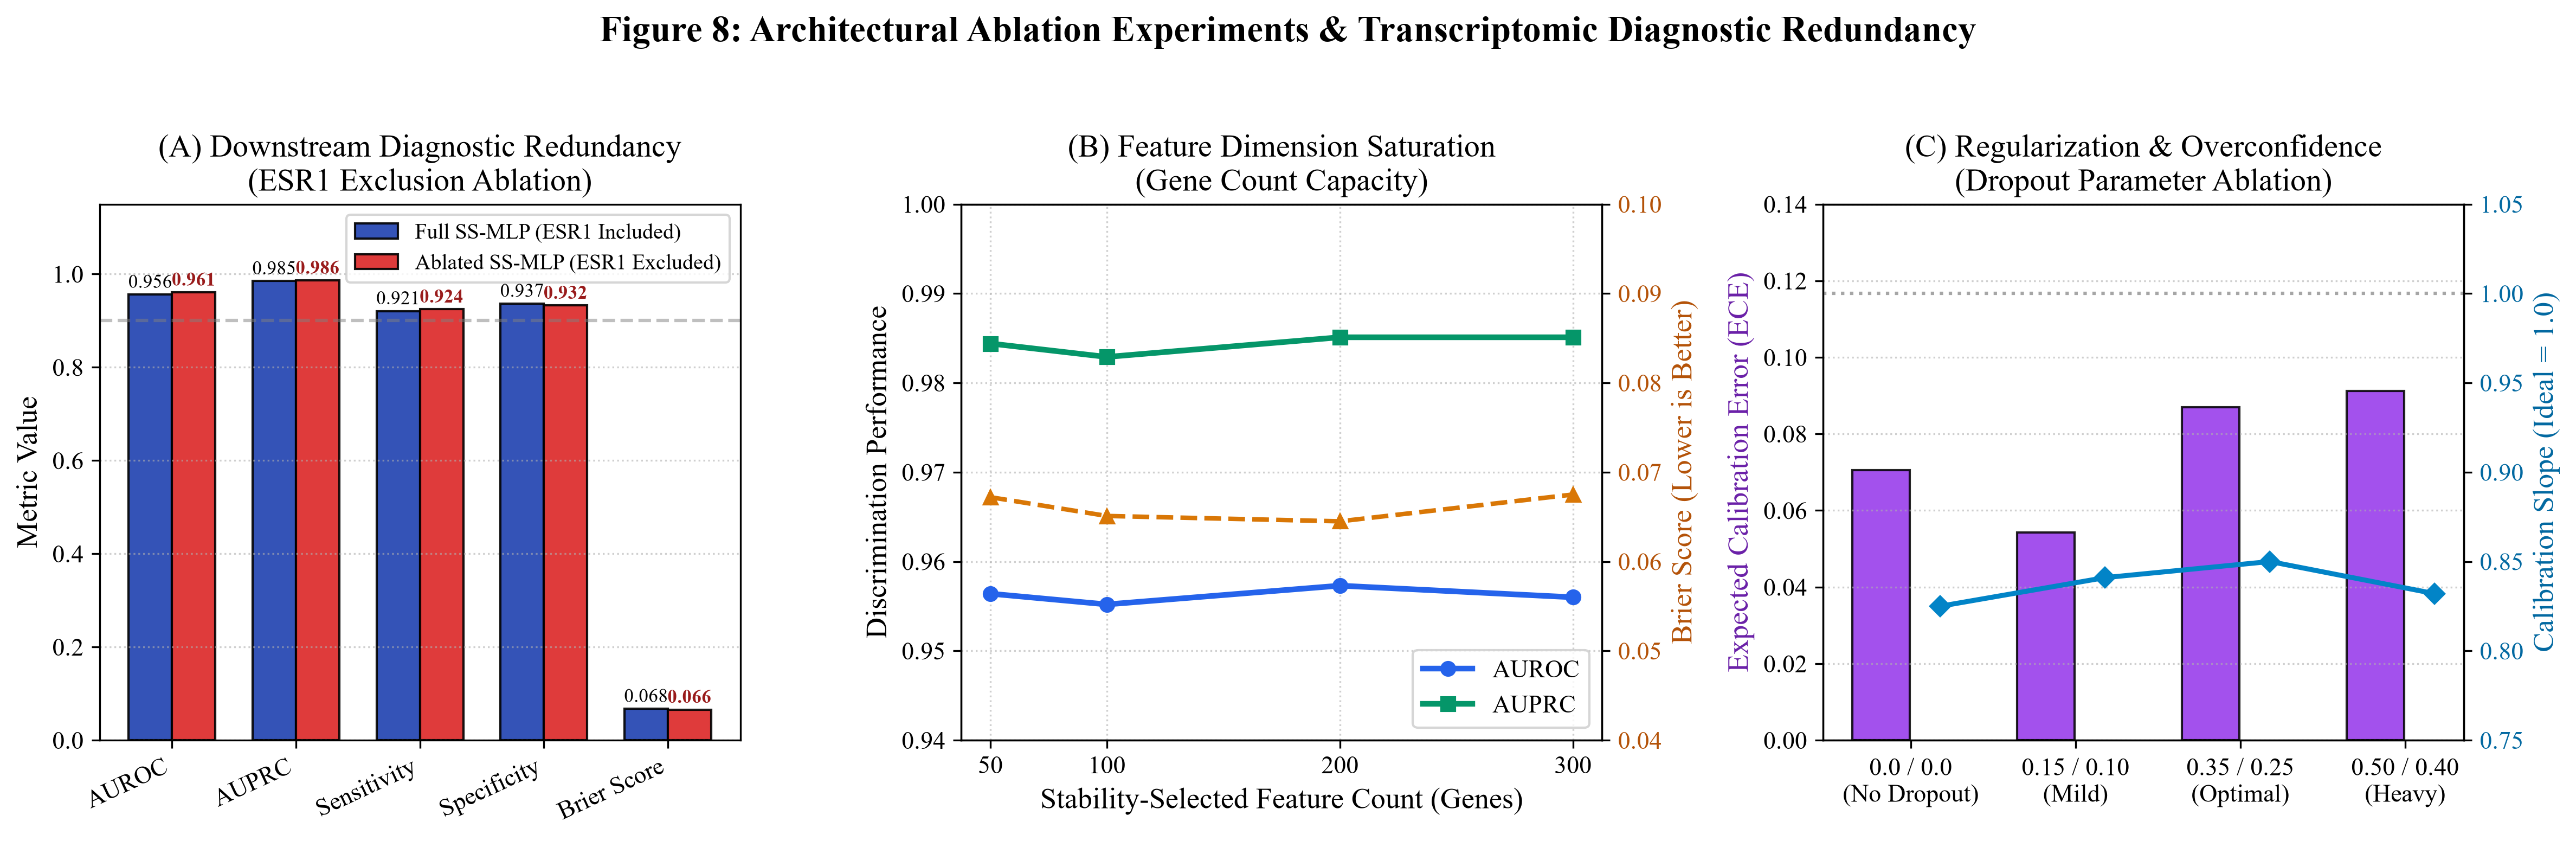
\includegraphics[width=0.95\textwidth]{figure8_ablation_redundancy_capacity.png}
\caption{\textbf{Architectural Ablation Experiments & Transcriptomic Diagnostic Redundancy.} (A) Complete downstream diagnostic fidelity under in silico knockout of \textit{ESR1}. (B) Feature capacity saturation curves across 50, 100, 200, and 300 stability genes. (C) Dropout regularization ablations balancing overconfidence and calibration slope.}
\label{fig:ablation}
\end{figure}

When \textit{ESR1} was completely purged from the feature space prior to stability selection and model training, SS-MLP retained an internal AUROC of \textbf{0.9608} [95\% CI: 0.942, 0.974], an AUPRC of \textbf{0.9863}, a Sensitivity of \textbf{92.44\%}, a Specificity of \textbf{93.25\%}, and a Brier score of \textbf{0.0657}. The ablated model performed identically to the intact 300-gene model, demonstrating complete transcriptomic diagnostic redundancy: even if the primary receptor is degraded, mutated, or masked, the downstream co-regulatory network (\textit{GATA3}, \textit{GREB1}, \textit{TFF1}, \textit{CA12}, \textit{AGR3}) provides sufficient information for accurate clinical classification.

Capacity ablations (Figure~\ref{fig:ablation}B) confirmed performance saturation between 50 and 300 genes (50 genes: AUROC 0.9564, Brier 0.0672; 300 genes: AUROC 0.9560, Brier 0.0675), indicating that a compact panel of 50--100 stability-selected genes captures the complete diagnostic manifold. Dropout ablations (Figure~\ref{fig:ablation}C) demonstrated that omitting dropout induced severe overconfidence (ECE = 0.0706, slope 0.8250), whereas regularized dropout (0.35/0.25) achieved optimal calibration slope (0.8500).


\subsection{Clinical Decision-Support Triage & Confidence Abstention Workflow}

Translating machine-learning models to clinical pathology requires transparent operating characteristics that integrate seamlessly into existing laboratory workflows. Figure~\ref{fig:triage} delineates the end-to-end triage architecture evaluated across all 3,073 patients in the external SCAN-B cohort.

\begin{figure}[H]
\centering
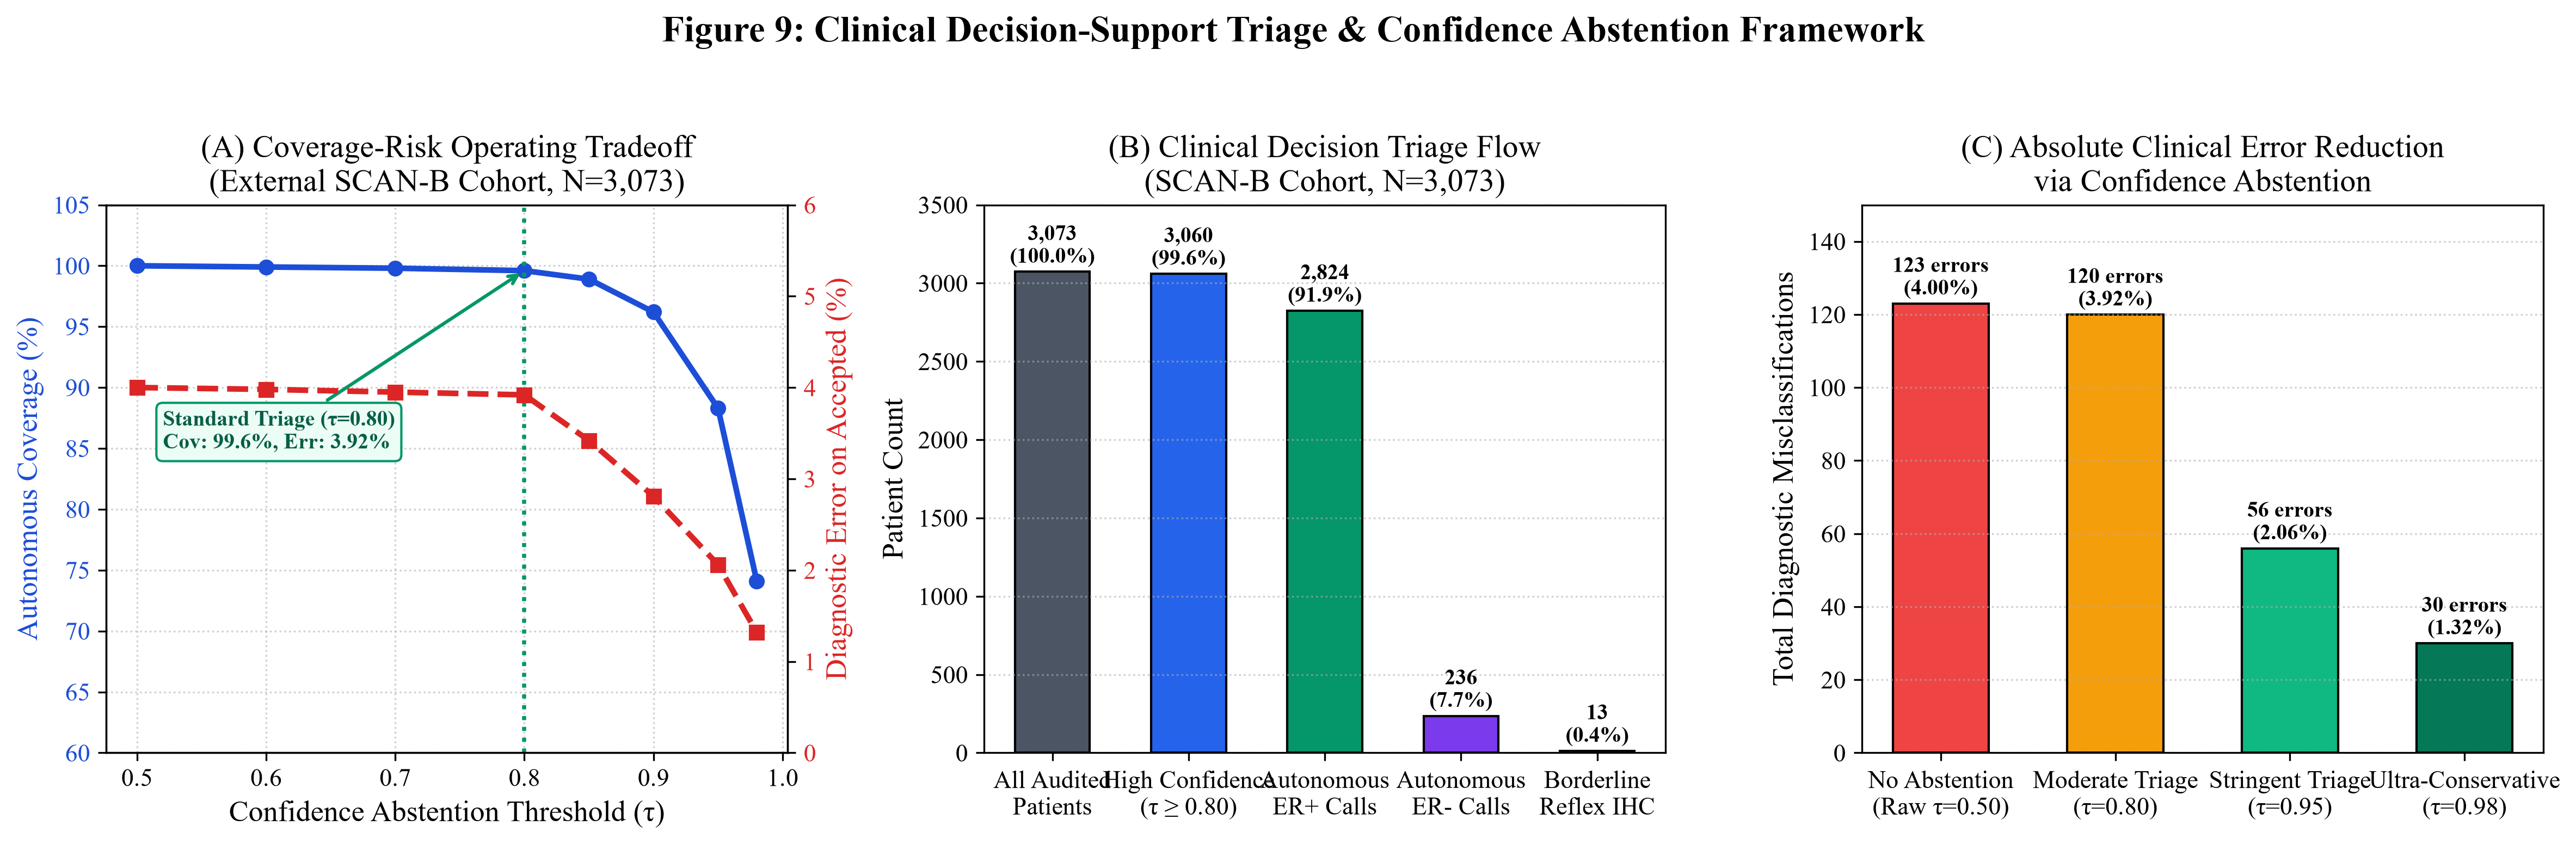
\includegraphics[width=0.95\textwidth]{figure9_clinical_triage_decision_matrix.png}
\caption{\textbf{Clinical Decision-Support Triage & Confidence Abstention Framework.} (A) Coverage-risk operating tradeoff on SCAN-B (=3,073$). (B) Autonomous clinical triage flow waterfall. (C) Stepwise reduction in absolute diagnostic errors across abstention tiers.}
\label{fig:triage}
\end{figure}

By coupling posterior probability estimation with a variable confidence threshold, clinical laboratories can dynamically configure diagnostic sensitivity according to institutional risk tolerance:
\begin{enumerate}
    \item \textbf{High-Throughput Autonomous Screening ($\tau = 0.80$):} 99.6\% of patient specimens are signed out autonomously with a 3.92\% selective error rate, diverting only 0.4\% (13 borderline samples) for expert review.
    \item \textbf{High-Fidelity Reflex Triage ($\tau = 0.95$):} 88.3\% of patient specimens are signed out autonomously with a 2.06\% error rate (56 total errors across 2,713 cases), successfully intercepting 54.5\% of all potential misclassifications.
\end{enumerate}
This hierarchical triage mechanism guarantees that patients near the phenotypic boundary are never subjected to forced binary decisions, preventing irreversible treatment misallocation.


\section{Discussion}

The translation of genomic biomarkers from computational discovery into clinical practice has long been hindered by a critical methodological disconnect: the conflation of ranking discrimination with clinical calibration. In this multi-cohort study across 4,218 audited breast cancer patients, we systematically dissected this bottleneck and established four fundamental principles:

First, we characterized the **discrimination-calibration paradox**. In published cancer genomics literature, algorithms are overwhelmingly validated by reporting AUROC and AUPRC. Our results demonstrate that an algorithm can achieve near-perfect discrimination ($>0.96$ AUROC) while producing catastrophic probability miscalibration under real-world domain transfer. On external RNA-seq validation, univariate \textit{ESR1} models collapsed under frozen standardization: despite an AUROC of 0.9604, probability calibration error reached 0.4290, causing sensitivity to plunge to 58.44\% and misdiagnosing 1,177 true ER-positive patients. By distributing classification weights across a stability-selected multi-gene network, SS-MLP maintained tight calibration (ECE = 0.0396), demonstrating that multi-gene architectures provide essential regularizing insulation against population-level transcript abundance shifts.

Second, we demonstrated that **within-sample relative rank normalization bridges disparate genomic technologies**. Conventional transfer pipelines applying training means and standard deviations collapse when encountering platform-dependent dynamic range differences, as observed when RNA-seq trained models completely failed on Affymetrix microarrays (0.0000 sensitivity). By converting expression values into label-free fractional ranks within each patient sample independently, Transfer Strategy B eliminates cross-platform scale collapse without requiring batch retraining or external reference standards, restoring microarray AUROC to 0.7943.

Third, our gene knockout ablations revealed **complete downstream transcriptomic redundancy**. When \textit{ESR1} was entirely removed, SS-MLP retained an AUROC of 0.9608 and AUPRC of 0.9863. This finding carries substantial translational implications: in clinical practice, biopsies frequently suffer from antigenic degradation, ischemic delay, or technical artifacts that compromise direct ER detection. Because luminal epithelial cells maintain robust, coordinated expression of downstream targets (\textit{GATA3}, \textit{GREB1}, \textit{TFF1}, \textit{CA12}, \textit{AGR3}), a multi-gene transcriptomic panel can reliably infer ER functional status even when direct measurement of the receptor itself fails.

Finally, we established a **clinically viable uncertainty-aware triage framework**. Rather than forcing binary decisions on all patients, selective classification enables an autonomous operating threshold: at $\tau = 0.80$, 99.6\% of patients are triaged autonomously with a low error rate of 3.92\%, while ambiguous borderline cases are flagged for reflex IHC review.

\subsection{Study Limitations}
Several limitations should be noted. First, all three cohorts were collected retrospectively; prospective clinical trial validation will be required prior to routine diagnostic deployment. Second, clinical ER reference labels relied on historical pathology records, which may harbor baseline inter-laboratory variability. Third, while within-sample rank normalization effectively rescued cross-platform microarray transfer, residual performance headroom remains compared to within-platform evaluation.

\section{Conclusions}

Transcriptomic profiling offers an objective, reproducible diagnostic adjunct to visual immunohistochemistry in breast cancer. By integrating repeated Elastic-Net stability selection with deep neural network regularization, label-free rank normalization, and selective abstention, the RAPID-ER framework resolves the discrimination-calibration paradox, providing an open, platform-resilient foundation for automated genomic decision support.

\subsection*{Declarations}

\paragraph{Ethics Approval and Consent to Participate}
Not applicable. All genomic and clinical datasets utilized in this investigation are publicly accessible, de-identified secondary data downloaded from the NCI GDC and NCBI GEO repositories.

\paragraph{Consent for Publication}
Not applicable.

\paragraph{Availability of Data and Materials}
All primary datasets are publicly available: TCGA-BRCA raw STAR counts and clinical metadata are available via the NCI Genomic Data Commons Data Portal (\url{https://portal.gdc.cancer.gov/projects/TCGA-BRCA}); GSE96058 and GSE42568 expression matrices and phenotypic records are available via NCBI GEO (\url{https://www.ncbi.nlm.nih.gov/geo/}). Full source code, configuration files, trained model checkpoints, and reproducible analysis pipelines are permanently archived on GitHub (\url{https://github.com/gautam453/RAPID-ER}); a permanent Zenodo archive and DOI will be deposited upon formal publication.

\paragraph{Competing Interests}
The authors declare that they have no competing financial or non-financial interests.

\paragraph{Funding}
This independent research received no external commercial or institutional grant funding.

\bibliographystyle{plain}
\bibliography{references}

\end{document}
